\documentclass[a4paper,11pt]{book}
%\documentclass[a4paper,twoside,11pt,titlepage]{book}
\usepackage{listings}
\usepackage[utf8]{inputenc}
\usepackage[spanish]{babel}
\usepackage[T1]{fontenc}

% \usepackage[style=list, number=none]{glossary} %
%\usepackage{titlesec}
%\usepackage{pailatino}

\decimalpoint
\usepackage{dcolumn}
\newcolumntype{.}{D{.}{\esperiod}{-1}}
\makeatletter
\addto\shorthandsspanish{\let\esperiod\es@period@code}
\makeatother



%\usepackage[chapter]{algorithm}
\RequirePackage{verbatim}
%\RequirePackage[Glenn]{fncychap}
\usepackage{fancyhdr}
\usepackage{graphicx}
\usepackage{afterpage}

\usepackage{longtable}
\usepackage[usenames]{color}

\usepackage[pdfborder={000}]{hyperref} %referencia

\usepackage{natbib} % Paquete para la gestión de la bibliografía

\usepackage{pdflscape}

\usepackage{multirow}
\usepackage{rotating}

\usepackage{glossaries}

\usepackage{float}

\usepackage{marvosym}

\usepackage{booktabs}

% ********************************************************************
% Re-usable information
% ********************************************************************
\newcommand{\myTitle}{Título del proyecto\xspace}
\newcommand{\myDegree}{Grado en ...\xspace}
\newcommand{\myName}{Nombre Apllido1 Apellido2 (alumno)\xspace}
\newcommand{\myProf}{Nombre Apllido1 Apellido2 (tutor1)\xspace}
\newcommand{\myOtherProf}{Nombre Apllido1 Apellido2 (tutor2)\xspace}
%\newcommand{\mySupervisor}{Put name here\xspace}
\newcommand{\myFaculty}{Escuela Técnica Superior de Ingenierías Informática y de
Telecomunicación\xspace}
\newcommand{\myFacultyShort}{E.T.S. de Ingenierías Informática y de
Telecomunicación\xspace}
\newcommand{\myDepartment}{Departamento de ...\xspace}
\newcommand{\myUni}{\protect{Universidad de Granada}\xspace}
\newcommand{\myLocation}{Granada\xspace}
\newcommand{\myTime}{\today\xspace}
\newcommand{\myVersion}{Version 0.1\xspace}


\hypersetup{
pdfauthor = {\myName (email (en) ugr (punto) es)},
pdftitle = {\myTitle},
pdfsubject = {},
pdfkeywords = {palabra_clave1, palabra_clave2, palabra_clave3, ...},
pdfcreator = {LaTeX con el paquete ....},
pdfproducer = {pdflatex}
}

%\hyphenation{}


%\usepackage{doxygen/doxygen}
%\usepackage{pdfpages}
\usepackage{url}
\usepackage{colortbl,longtable}
\usepackage[table,xcdraw]{xcolor}
\usepackage[stable]{footmisc}
%\usepackage{index}

\usepackage{amssymb}
\usepackage{pifont}
\newcommand{\cmark}{\ding{51}}
\newcommand{\xmark}{\ding{55}}

%\makeindex
%\usepackage[style=long, cols=2,border=plain,toc=true,number=none]{glossary}
% \makeglossary

% Definición de comandos que me son tiles:
%\renewcommand{\indexname}{Índice alfabético}
%\renewcommand{\glossaryname}{Glosario}

\pagestyle{fancy}
\fancyhf{}
\fancyhead[LO]{\leftmark}
\fancyhead[RE]{\rightmark}
\fancyhead[RO,LE]{\textbf{\thepage}}
\renewcommand{\chaptermark}[1]{\markboth{\textbf{#1}}{}}
\renewcommand{\sectionmark}[1]{\markright{\textbf{\thesection. #1}}}

\setlength{\headheight}{1.5\headheight}

\newcommand{\HRule}{\rule{\linewidth}{0.5mm}}
%Definimos los tipos teorema, ejemplo y definición podremos usar estos tipos
%simplemente poniendo \begin{teorema} \end{teorema} ...
\newtheorem{teorema}{Teorema}[chapter]
\newtheorem{ejemplo}{Ejemplo}[chapter]
\newtheorem{definicion}{Definición}[chapter]

\definecolor{gray97}{gray}{.97}
\definecolor{gray75}{gray}{.75}
\definecolor{gray45}{gray}{.45}
\definecolor{gray30}{gray}{.94}

\lstset{ frame=Ltb,
     framerule=0.5pt,
     aboveskip=0.5cm,
     framextopmargin=3pt,
     framexbottommargin=3pt,
     framexleftmargin=0.1cm,
     framesep=0pt,
     rulesep=.4pt,
     backgroundcolor=\color{gray97},
     rulesepcolor=\color{black},
     %
     stringstyle=\ttfamily,
     showstringspaces = false,
     basicstyle=\scriptsize\ttfamily,
     commentstyle=\color{gray45},
     keywordstyle=\bfseries,
     %
     numbers=left,
     numbersep=6pt,
     numberstyle=\tiny,
     numberfirstline = false,
     breaklines=true,
   }
 
% minimizar fragmentado de listados
\lstnewenvironment{listing}[1][]
   {\lstset{#1}\pagebreak[0]}{\pagebreak[0]}

\lstdefinestyle{CodigoC}
   {
	basicstyle=\scriptsize,
	frame=single,
	language=C,
	numbers=left
   }
\lstdefinestyle{CodigoC++}
   {
	basicstyle=\small,
	frame=single,
	backgroundcolor=\color{gray30},
	language=C++,
	numbers=left
   }

 
\lstdefinestyle{Consola}
   {basicstyle=\scriptsize\bf\ttfamily,
    backgroundcolor=\color{gray30},
    frame=single,
    numbers=none
   }


\newcommand{\bigrule}{\titlerule[0.5mm]}


%Para conseguir que en las páginas en blanco no ponga cabecerass
\makeatletter
\def\clearpage{%
  \ifvmode
    \ifnum \@dbltopnum =\m@ne
      \ifdim \pagetotal <\topskip
        \hbox{}
      \fi
    \fi
  \fi
  \newpage
  \thispagestyle{empty}
  \write\m@ne{}
  \vbox{}
  \penalty -\@Mi
}
\makeatother

\usepackage{pdfpages}


\makeglossaries


\newglossaryentry{world_wide_web}
{
    name=World Wide Web,
    description={La World Wide Web (W3) fue desarrollada por un conjunto de personas, de entre las que destaca Tim Berners-Lee, a finales de la década de los ochenta. El motivo por el que surgió este desarrollo fue el interés por parte del CERN de poder compartir sus investigaciones con el resto del mundo y por tanto mejorar la comunicación en el mundo investigador.}
}

\newglossaryentry{bot}
{
    name=bot,
    description={Un bot \footnote{https://dictionary.cambridge.org/es-LA/dictionary/english/bot} es un programa informático que trabaja de forma autónoma.}
}

\newglossaryentry{chatbot}
{
    name=chatbot,
    description={Un chatbot \footnote{https://dictionary.cambridge.org/es-LA/dictionary/english/chatbot} es un programa informático diseñado para tener una conversación con un humano, especialmente a través de Internet.}
}

\newglossaryentry{front-end}
{
    name=front-end,
    description={El front-end es la capa que se encuentra por encima del \gls{back-end}. Es la capa visible para el usuario y también es con la que interactúa. Debido a se interactúa con ella debe cumplir unos estándares de usabilidad y estética. Los principales lenguajes de programación con los que se implementa esta capa son: Javascript, CSS y HTML.}
}

\newglossaryentry{back-end}
{
    name=back-end,
    description={El back-end es la capa que se encuentra por debajo del \gls{front-end}. Es la capa no visible para el usuario. En ella se encuentra el funcionamiento de la aplicación, incluyendo servidores y bases de datos. No existe un lenguaje de programación específico para esta capa.}
}

\newglossaryentry{full_stack}
{
    name=Full Stack,
    description={La programación Full Stack abarca tanto la programación del \gls{front-end} como la del \gls{back-end}. Los profesionales de esta programación se denominan programadores Full Stack y tienen las habilidades necesarias para administrar un proyecto completo.}
}

\newglossaryentry{responsive}
{
    name=responsive,
    description={Según Brett S. Gardner \cite{RefWorks:RefID:34-2011responsive}, el diseño responsive de las páginas web permite crear una única página web que es capaz de adaptarse a la interfaz y al contenido de la misma para poder ser visible en distintos dispositivos (móviles, tablets y ordenadores). Este diseño permite mejorar la experiencia del usuario. Actualmente el diseño responsive se implementa a través del lenguaje CSS, en concreto con su versión CSS3, la cuál tiene un enfoque centrado en el usuario permitiendo el diseño de aplicaciones web dinámicas.}
}

\newglossaryentry{API REST}
{
    name=API REST,
    description={Una API REST es un \gls{API} que sigue los principios de diseño de REST. El principal objetivo de estos principios es tener una \gls{API} que posibilite la separación entre cliente y servidor, para ello algunos de sus principios son por ejemplo: tener un interfaz uniforme, es decir, todas las solicitudes hacia un recurso de la API son siempre iguales; o no tener estado, es decir, la API no guarda información, todas la información necesaria para resolver la solicitud debe estar contenida en la misma.}
}

\newglossaryentry{API}
{
    name=API,
    description={Según la página web de IBM \cite{RefWorks:RefID:33-2021-API}, una API o interfaz de programación de aplicaciones, es un conjunto de reglas que determinan cómo las aplicaciones o los dispositivos pueden conectarse y comunicarse entre sí.}
}

\newglossaryentry{Siracusa}
{
    name=Siracusa,
    description={Siracusa es una ciudad de Italia, situada en la costa sudeste de la isla de Sicilia, famosa como centro cultural desde la Antigua Grecia.}
}

\newglossaryentry{Github}
{
    name=Github,
    description={Github es una plataforma donde multitud de personas y empresas desarrollan software. Esta plataforma permite la comunicación e interacción de la comunidad de desarrolladores de software. Los proyectos se alojan en lo que se denominan repositorios, los cuáles pueden ser públicos o privados. Cada repositorio tiene un control de versiones mediante Git.}
}




\begin{document}
\begin{titlepage}
 
 
\newlength{\centeroffset}
\setlength{\centeroffset}{-0.5\oddsidemargin}
\addtolength{\centeroffset}{0.5\evensidemargin}
\thispagestyle{empty}

\noindent\hspace*{\centeroffset}\begin{minipage}{\textwidth}

\centering

\includegraphics[width=0.9\textwidth]{imagenes/logo_ugr.jpg}\\[1.4cm]

\textsc{ \Large TRABAJO FIN DE GRADO\\[0.2cm]}
\textsc{ INGENIERÍA EN INFORMÁTICA}\\[1cm]
% Upper part of the page
% 
% Title
{\Huge\bfseries Agente conversacional multiedad\\
}
\noindent\rule[-1ex]{\textwidth}{3pt}\\[3.5ex]
{\large\bfseries Agente conversacional enfocada a la enseñanza}
\end{minipage}

\vspace{2.5cm}
\noindent\hspace*{\centeroffset}\begin{minipage}{\textwidth}
\centering

\textbf{Autor}\\ {Mario Carmona Segovia}\\[2.5ex]
\textbf{Directora}\\
{Rocío Celeste Romero Zaliz}\\[2cm]

\includegraphics[width=0.3\textwidth]{imagenes/etsiit_logo.png}\\[0.1cm]
\textsc{Escuela Técnica Superior de Ingenierías Informática y de Telecomunicación}\\
\textsc{---}\\
Granada, julio de 2021
\end{minipage}
%\addtolength{\textwidth}{\centeroffset}
%\vspace{\stretch{2}}
\end{titlepage}



\chapter*{}
%\thispagestyle{empty}
%\cleardoublepage

%\thispagestyle{empty}

%\cleardoublepage
\thispagestyle{empty}

\begin{center}
{\large\bfseries Título del Proyecto: Subtítulo del proyecto}\\
\end{center}
\begin{center}
Mario Carmona Segovia\\
\end{center}

%\vspace{0.7cm}
\noindent{\textbf{Palabras clave}: palabra\_clave1, palabra\_clave2, palabra\_clave3, ......}\\

\vspace{0.7cm}
\noindent{\textbf{Resumen}}\\

Poner aquí el resumen.
\cleardoublepage


\thispagestyle{empty}


\begin{center}
{\large\bfseries Project Title: Project Subtitle}\\
\end{center}
\begin{center}
Mario Carmona Segovia\\
\end{center}

%\vspace{0.7cm}
\noindent{\textbf{Keywords}: Keyword1, Keyword2, Keyword3, ....}\\

\vspace{0.7cm}
\noindent{\textbf{Abstract}}\\

Write here the abstract in English.

\chapter*{}
\thispagestyle{empty}

\noindent\rule[-1ex]{\textwidth}{2pt}\\[4.5ex]

Yo, \textbf{Mario Carmona Segovia}, alumno de la titulación Grado en Ingeniería Informática de la \textbf{Escuela Técnica Superior
de Ingenierías Informática y de Telecomunicación de la Universidad de Granada}, con DNI 45922466, autorizo la
ubicación de la siguiente copia de mi Trabajo Fin de Grado en la biblioteca del centro para que pueda ser
consultada por las personas que lo deseen.

\vspace{6cm}

\noindent Fdo: Mario Carmona Segovia

\vspace{2cm}

\begin{flushright}
Granada a X de mes de 201 .
\end{flushright}


\chapter*{}
\thispagestyle{empty}

\noindent\rule[-1ex]{\textwidth}{2pt}\\[4.5ex]

D. \textbf{Rocío Celeste Romero Zaliz}, Profesora del Departamento de Ciencias de la Computación e Inteligencia Artificial de la Universidad de Granada.

\vspace{0.5cm}

\textbf{Informan:}

\vspace{0.5cm}

Que el presente trabajo, titulado \textit{\textbf{Título del proyecto, Subtítulo del proyecto}},
ha sido realizado bajo su supervisión por \textbf{Mario Carmona Segovia}, y autorizamos la defensa de dicho trabajo ante el tribunal
que corresponda.

\vspace{0.5cm}

Y para que conste, expiden y firman el presente informe en Granada a X de mes de 201 .

\vspace{1cm}

\textbf{La directora:}

\vspace{5cm}

\noindent \textbf{Nombre Apellido1 Apellido2 (tutor1) \ \ \ \ \ Nombre Apellido1 Apellido2 (tutor2)}

\chapter*{Agradecimientos}
\thispagestyle{empty}

       \vspace{1cm}


Poner aquí agradecimientos...


%\frontmatter
\tableofcontents
\listoffigures
\listoftables
%
%\mainmatter
%\setlength{\parskip}{5pt}

\chapter{Introducción}

La motivación de los seres humanos por difundir los conocimientos existentes a la mayor cantidad de personas posible ha existido desde que el ser humano es ser humano. Por supuesto, en sus inicios esta difusión se producía a una menor escala, principalmente a una escala local, de forma oral y a un ritmo muy lento. Además, eran conocimientos básicos, útiles sobre todo para la realización de las tareas diarias.

Conforme ha ido evolucionando el ser humano, esta difusión de conocimiento ha evolucionado junto a él. Por ejemplo, con hitos como la invención de la escritura, la difusión pudo aumentar su ritmo, tener un rango de alcance un poco mayor, y sobre todo posibilitó difundir conocimientos más complejos.

Aunque la evolución de la difusión de conocimiento se ha ido produciendo paulatinamente, el ritmo al que lo ha hecho no ha sido algo destacable, ya que siempre han existido dos grandes impedimentos. Por un lado, la falta de educación en la mayor parte de la población, lo que provoca la ausencia de motivación por aprender. Y, por otro lado, la dificultad de difusión, puesto que a pesar de haber tenido algunos avances gracias a hitos en la historia de la humanidad, tales como la invención de la escritura, mencionado anteriormente, o el aumento del tráfico mundial.

La falta de educación en la población se ha ido disipando en las últimas décadas, al hacer más fácil el acceso a los conocimientos.

El hito que si supuso un boom en la difusión de conocimiento fue la creación de la \gls{world_wide_web}. Este hito no solamente supuso un avance enorme en el aumento del tráfico de información mundial, sino también hizo aún más fácil el acceso de cualquier persona al conocimiento, sobre todo cuando se extendió el uso de ordenadores personales.

Después del último hito se ha llegado a tal punto de difusión, que el aumento de la difusión ha pasado a un segundo plano y ahora los esfuerzos se están centrando en hacer que la difusión sea más natural para aquellas personas que consultan la información.

Una de las posibles ramas para difundir conocimiento de forma natural es mediante la conversación con un \gls{bot}, o también llamados chatbots.

\section{Motivación y objetivos}

El potencial que tienen los chatbots como herramienta para la difusión de conocimientos de modo natural ha motivado la creación de este proyecto.

Además de lo anteriormente dicho, también ha motiva el desarrollo de este proyecto, la posible aplicación del mismo para los eventos de "La Noche Europea de l@s Investigador@s", en los cuales se realizan distintas actividades culturales. Una de estas actividades es el fomento sobre el mundo de la informática, acercando a todo tipo de personas a las posibilidades que tiene la informática de ser usada en las tareas que ellos llevan a cabo o que pretenden iniciar.

El principal objetivo de este proyecto es facilitar la creación de chatbots orientados a la difusión de información sobre una cierta temática y que además disponen de una cierta personalización a la hora de conversar dependiendo de ciertas características de la persona con la que se conversa.

\section{Descripción del proyecto}

El nombre que se le ha dado al chatbot es Sara. El nombre ha tenido como origen el nombre de la ciudad gls{Siracusa} en siciliano, Sarausa. El motivo de elegir este nombre es mi interés por la historia antigua. Además, idealmente el nombre de un chatbot debe ser corto y fácil de recordar, y el nombre de Sara lo cumple perfectamente.

El proyecto consiste en el desarrollo de una aplicación cliente-servidor. La aplicación es desplegada en la nube. Mi papel en este proyecto será parecida a la de un programador \gls{full_stack}.

En cuanto a la parte del cliente, es adaptable a cualquier tipo de \gls{front-end} o interfaz siguiendo un diseño \gls{responsive}. Esta parte en todo momento busca ser lo más cómoda y accesible posible para el usuario.

Pero la parte del servidor o \gls{back-end} es la más importante de esta aplicación, ya que contiene toda la lógica del chatbot. La parte del servidor es una \gls{API REST}, la cual permite la adaptabilidad de la interfaz, separando cliente y servidor.

El proyecto en su totalidad ha sido alojado en un repositorio de \gls{Github}, cuyo nombre es \href{https://github.com/Mario-Carmona/SARA_Chatbot}{SARA\_Chatbot}. Este repositorio se ha mantenido en privado durante el desarrollo del proyecto, pero tras su finalización se pondrá en público para su libre uso y consulta. Durante el desarrollo del proyecto se ha seguido una metodología de desarrollo ágil, la cual permite ir generando prototipos de la aplicación durante el desarrollo del proyecto, los cuales se pueden evaluar para tener en cuenta los fallos para futuros prototipos.

\section{Estructura de la memoria}

\begin{itemize}
\item \textbf{Capítulo 1. Introducción:} Breve introducción al proyecto, indicando además los motivos por los que se ha desarrollado y una breve descripción técnica del proyecto.
\end{itemize}

\section{Licencia}

********************************


\chapter{Estado del Arte}

\section{Análisis del Estado del Arte} \label{sec:analisis_estado_arte}

Los chatbots son \gls{agentes_conversacionales} que pueden interactuar, a través de voz o texto, con los usuarios a través de lenguajes naturales \cite{RefWorks:RefID:36-luo2022critical}. El auge de esta tecnología en los últimos años es debido a que puede ser utilizada como mano de obra a un coste menor en una amplia gama de campos. Tal y como se indica en \cite{RefWorks:RefID:37-adamopoulou2020overview} los chatbots no están diseñados solamente para imitar y entretener a los humanos, sino que también puede diseñarse para actividades como la atención al cliente, la asistencia personal o la pedagogía entre otras. Y no hay mejor forma de asegurar el potencial de los chatbots que mostrando el aumento de inversión en \gls{IA} en el campo de las telecomunicaciones (Figura \ref{fig:inversion_chatbot}) o mostrando el aumento de publicaciones sobre chatbots (Figura \ref{fig:publicaciones_chatbot}); y viendo qué empresas están apostando por esta tecnología, como pueden ser cinco grandes empresas tecnológicas como son Google, Apple, Facebook, Microsoft y Amazon. Aunque basándonos en este párrafo de la sensación de que todas las empresas deberían disponer de chatbots, esta tecnología necesita de cierta planificación y comprensión de la tecnología, pues requiere de una gran inversión inicial, dado su gran requerimiento de información para funcionar de forma correcta.

\begin{figure}[h]
\centering
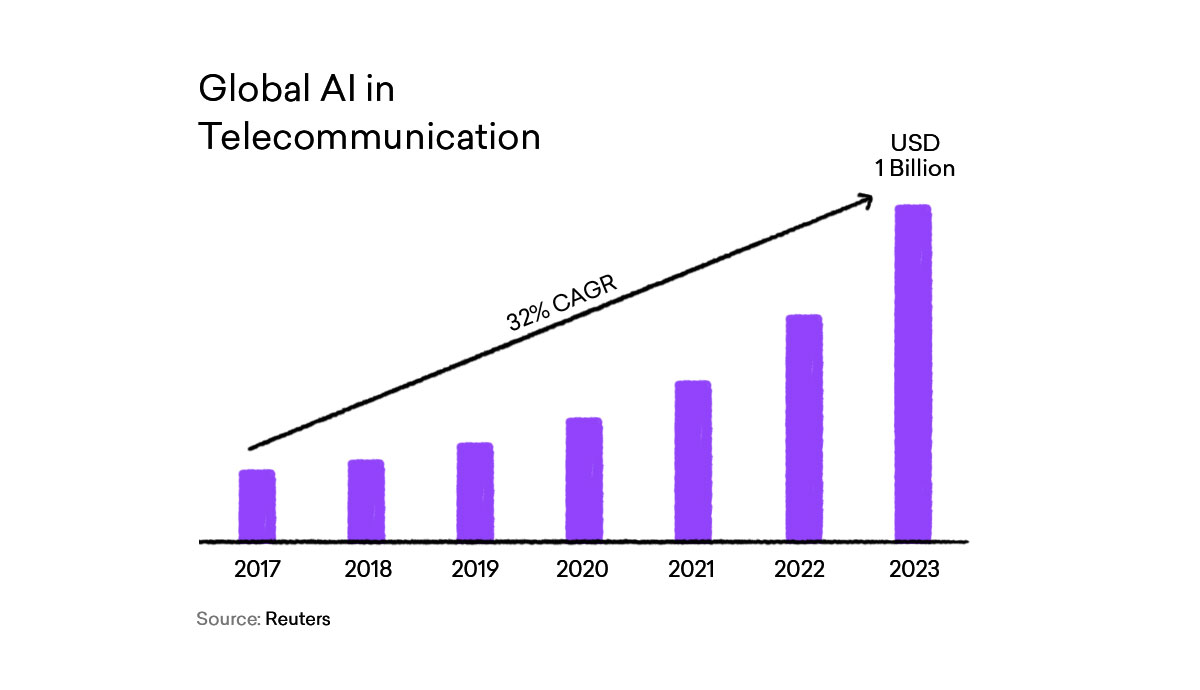
\includegraphics[width=1.0\textwidth]{imagenes/02_EstadoDelArte/inversion_chatbots.jpg}
\begin{center}
Fuente: \url{https://es.aivo.co/blog/chatbots-in-telecom}
\end{center}
\caption{Estimación de la inversión en IA en el campo de las telecomunicaciones}
\label{fig:inversion_chatbot}
\end{figure}

\begin{figure}[h]
\centering
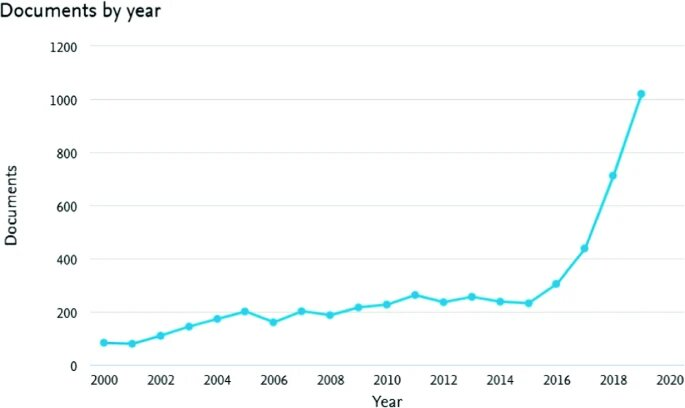
\includegraphics[width=1.0\textwidth]{imagenes/02_EstadoDelArte/publicaciones_chatbots.jpg}
\begin{center}
Fuente: \url{https://link.springer.com/chapter/10.1007/978-3-030-49186-4_31}
\end{center}
\caption{Historial de las publicaciones sobre temas relacionados con chatbots}
\label{fig:publicaciones_chatbot}
\end{figure}

Aunque es una tecnología en auge y con mucho potencia en este momento, hay aspectos de ella que todavía no están lo suficientemente desarrollados como para decir que se trata de una tecnología del todo madura. Estas carencias están sobre todo enfocadas en tres puntos.
En primer lugar, nos encontramos con el problema que aparece nada más empezar, y es la carencia de un esquema de clasificación de chatbots, dado que no se ha definido una clasificación global. La clasificación más extendida es la clasificación según el mecanismo de recuperación y de generación de respuestas, donde destacan los chatbots que hacen uso de bases de conocimientos estáticas, es decir, chatbots basados en reglas; y los chatbots que hacen uso de mecanismos de aprendizaje e inferencia adaptativos, es decir, los chatbots basados en \newline\gls{IA}, los cuales son el objetivo de la mayoría de los desarrollos actuales. En segundo punto, las revisiones están desactualizadas en el ámbito de la generación de respuestas dado el rápido avance de las técnicas computacionales. En tercer punto, también las revisiones no están muy centradas en la aplicación empresarial de los chatbots ni en su usabilidad, sino que más bien están centradas en el aspecto técnico, lo cual complica su desarrollo por parte de trabajadores ajenos al mundo de la informática y/o de la \gls{IA}.

La estructura de los chatbots ha ido evolucionando y extendiéndose. Originalmente, la estructura de los chatbots era la descrita por Abdul-Kader y Woods \cite{RefWorks:RefID:36-luo2022critical}, donde se podía reconocer tres componentes: interfaz, un clasificador y un graphmaster. Esta estructura está muy desactualizada a día de hoy, ya que en la estructura original la interfaz solo tenía previstas entradas en forma de texto, pero hoy en día las entradas son de tipo multimedia, por lo que es necesario actualizar la interfaz a una interfaz multimedia, y añadir un nuevo componente a la estructura, encargado de manejar esas entradas multimedia y convertirlas en entradas de texto que se puedan manejar para generar respuestas; además dado el auge de los chatbots basados en generación, a día de hoy el componente del graphmaster no tiene sentido, dado que las respuestas se generan utilizando modelos pre entrenados realizando inferencias basándose en las entradas, por lo que tener un manejador para el almacenamiento de conocimiento deja de tener sentido. Por lo tanto, en la estructura el graphmaster debe ser actualizado por un modelo generador de respuestas. Aplicando todas estas actualizaciones sobre la estructura original de Abdul-Kader y Woods, obtenemos la estructura actual de los chatbots, que se muestra en la Figura \ref{fig:estructura_state_of_art}. Finalmente, tenemos cuatro componentes: la interfaz, un procesador multimedia, un análisis de entrada multimodal y un generador de respuestas.

\begin{figure}[h]
\centering
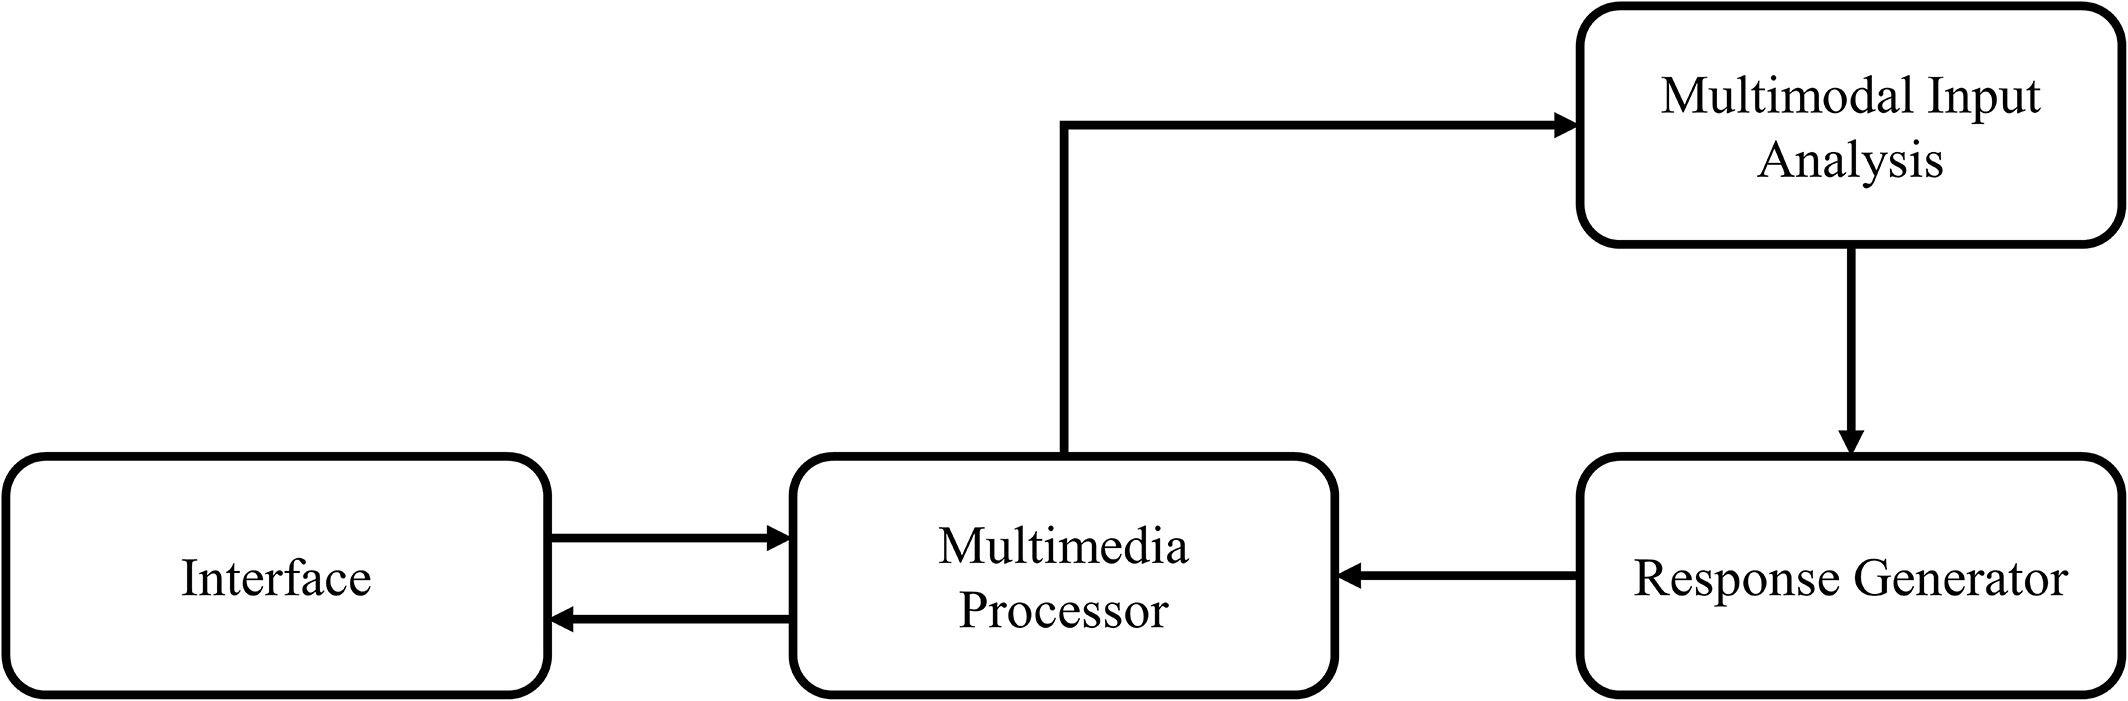
\includegraphics[width=0.8\textwidth]{imagenes/02_EstadoDelArte/estructura_state_of_art.jpg}
\begin{center}
Fuente: A critical review of state-of-the-art chatbot designs and applications \cite{RefWorks:RefID:36-luo2022critical}
\end{center}
\caption{Estructura de los chatbots actuales}
\label{fig:estructura_state_of_art}
\end{figure}

Un componente que se muestra en la Figura \ref{fig:estructura_state_of_art} y que no se ha mencionado explícitamente cuál es su labor es el análisis de entrada multimodal. Este análisis efectúa un pretratamíento de los datos de entrada, hoy en día se intenta mejorar este componente con \gls{NLU} (NLU).

En el caso de los chatbots basados en la recuperación, el generador de respuestas desempeña el mismo papel que el graphmaster, ya que almacena y recupera las respuestas; mientras que en el caso de los chatbots basados en la generación, genera una salida a partir de la entrada que ha sido transferida desde la unidad de pretratamiento \cite{RefWorks:RefID:36-luo2022critical}.

Centrándonos en el componente del generador de respuestas, a día de hoy se utilizan distintas técnicas para implementar este componente. Las técnicas más destacadas son las siguientes:

\begin{itemize}
\item \textbf{Template:} Esta técnica se compone de patrones y plantillas formando pares con ellos. Para generar las respuestas se busca el patrón que más concuerde con la entrada recibida, y una vez se haya elegido un patrón se devuelve la plantilla asociada al mismo. El lenguaje que más destaca en esta técnica es AIML \footnote{\url{http://www.aiml.foundation}}. La desventaja de tener que crear los archivos AIML se puede suplir mediante la extracción automática de conocimientos, reduciendo el trabajo manual. Los chatbots basados en plantillas son sencillos de producir, por lo tanto, son una opción popular para chatbots sencillos a pequeña escala.
\item \textbf{Corpus:} Son una buena técnica como alternativa a los templates cuando se están construyendo chatbots a gran escala, debido a que con los templates al aumentar de escalas aumenta el número de patrones y trae consigo búsquedas más lentas lo que ralentiza la generación de respuestas. Existen dos tipos de chatbots basados en Corpus, un tipo de chatbots basados en corpus que no selecciona cuidadosamente el conocimiento y otro que si lo hace. El tipo que selecciona cuidadosamente el conocimiento se puede implementar mediante bases de datos o mediante modelos de ontología, los modelos de ontología tienen una gestión más flexible del conocimiento que las bases de datos, la generación en este tipo de chatbots se realiza también con búsqueda pero esta vez en las estructuras mencionadas anteriormente. El tipo que no selecciona cuidadosamente el conocimiento transforma las palabras en vectores que representan los significados semánticos de las palabras en un espacio multidimensional, la generación en este tipo de chatbots se realiza mediante el cálculo de la distancia entre los pares de entrada del usuario y de consulta-respuesta, se empareja la consulta con la menor distancia y se selecciona su correspondiente respuesta como salida. Debido a la gran capacidad de gestión del conocimiento, varias aplicaciones que requieren un conocimiento formal del dominio utilizan chatbots basados en corpus \cite{RefWorks:RefID:36-luo2022critical}.
\item \textbf{Intent:} Los chatbots basados en intenciones se emplean ampliamente para los sistemas orientados a tareas que presentan diálogos de varios turnos \cite{RefWorks:RefID:36-luo2022critical}. Una intención representa un mapeo entre lo que dice el usuario y la acción que debería ejecutar el chatbot. El emparejamiento de las entradas con las distintas intenciones se hace de una forma distinta a la vista anteriormente, dado que ahora debemos emparejar los elementos semántico en vez de la frase completa. Puesto que la entrada es una frase, en el caso de esta técnica es necesario añadir adicionalmente un componente de análisis de entrada multimodal (SLU), dentro de él se efectúa un análisis semántico de las entradas, para este análisis se suelen usar \gls{NLU}. Una vez tenemos los elementos semánticos de la entrada se procede a emparejar la entrada con una intención o dicho de otra manera, se procede a efectuar una clasificación para saber a qué intención pertenece la entrada, esta clasificación se suele hacer mediante técnicas de aprendizaje automático. Otra característica de este tipo de chatbots es la existencia de estados, debido a que son chatbots orientados a tareas; los cuales determinan el momento de la conversación en el que nos encontramos, que intenciones han sido ejecutadas, y cuáles pueden ser elegidas para ejecutar posteriormente. El manejo de los estados se compone de dos tareas, por un lado, la obtención del estado actual del diálogo, para lo cual se utilizan técnicas de \gls{DST}; y, por otro lado, el procesamiento del estado del diálogo para determinar a que estado se va a pasar el diálogo, para esta tarea se utilizan técnicas de \gls{DPO}. Las dos técnicas mencionadas son necesarias para establecer la secuencia de los diálogos. Las bases de conocimiento de los generadores de respuestas en los chatbots basados en intenciones están compuestas principalmente de frases de entrenamiento, intenciones y respuestas. Para generar las respuestas se analiza semánticamente las entradas en el módulo SLU, posteriormente se emplea el módulo \gls{DST}para estimar el estado de los diálogos actuales y finalmente se emplea el módulo \gls{DPO} para determinar las acciones y respuestas.

Para un mejor entendimiento de esta compleja estructura se dispone de la Figura \ref{fig:estructura_intent}.

\begin{figure}[h]
\centering
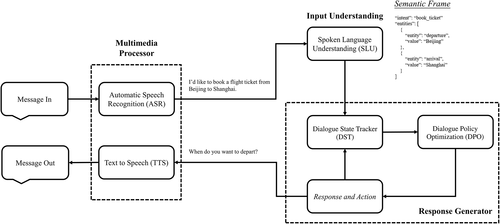
\includegraphics[width=0.8\textwidth]{imagenes/02_EstadoDelArte/estructura_intent.png}
\begin{center}
Fuente: A critical review of state-of-the-art chatbot designs and applications \cite{RefWorks:RefID:36-luo2022critical}
\end{center}
\caption{Estructura de los chatbots basados en intenciones}
\label{fig:estructura_intent}
\end{figure}

Muchas de las grandes plataformas actualmente están orientadas a la creación de chatbots de este tipo, como puede ser la plataforma de Google con Dialogflow \footnote{\url{https://dialogflow.cloud.google.com}} (originalmente llamado Api.ai) o la plataforma de código abierto de Rasa. \footnote{\url{https://rasa.com/}}.
\item \textbf{Red neuronal recurrente (RNN):} Los chatbots creados con esta técnica dejarán de estar basados en la recuperación, como pasaba en las tres anteriores técnicas, si no que estarán basados en la generación, pero esto que quiere decir, en definitiva quiere decir que la generación de las respuestas no se realizará mediante búsquedas en alguna estructura y sustitución mediante pares consulta-respuesta. La generación de las respuestas se efectúa mediante inferencias con modelos de redes neuronales recurrentes. Estos chatbots, a diferencia de los chatbots basados en intenciones, no están orientados a las tareas y esto deriva del problema que conllevan las redes neuronales, y no es otro que las redes convierten al chatbot en una \gls{caja_negra}, esto quiere decir que la respuesta del chatbot ante cierta entrada es incierta incluso para su creador, este inconveniente se convierte en una ventaja si orientamos a los chatbots al chat, dado que esta incertidumbre en la respuesta da una gran sensación de naturalidad y creatividad durante la conversación, por lo que son apropiados para actividades relacionadas con el entretenimiento y la salud mental entre otras. Estos chatbots se han visto muy potenciados en los últimos años debido al rápido desarrollo del aprendizaje profundo. Uno de los mayores hitos en el aprendizaje profundo ha sido la creación de GPT-3 \footnote{\url{https://openai.com/blog/openai-api}} creado por la empresa OpenAI, el cual es un nuevo modelo de inteligencia artificial que permite generar lenguaje escrito. Como se ha mencionado anteriormente, ya no se realiza recuperación para la generación de respuestas, por lo tanto, las bases de conocimiento de los chatbots basados en RNN estarán compuestas de los conjuntos de datos de entrenamiento. El resultado de los chatbots basados en la generación depende de la especificación del modelo, los conjuntos de datos de entrenamiento, el proceso de entrenamiento y la entrada del usuario \cite{RefWorks:RefID:36-luo2022critical}.
\item \textbf{Aprendizaje por refuerzo (RL):} Este tipo de chatbots suelen estar basados en la recuperación y utilizan plenamente el contexto de entrada para la búsqueda de respuestas óptimas \cite{RefWorks:RefID:36-luo2022critical}. Dado que se basan en la recuperación, en sus bases de conocimientos hay pares de consulta-respuesta predefinidos. El método RL se basa principalmente en el \gls{Markov}. Al igual que pasaba en los chatbots basados en templates, en los chatbots basados en RL se usan representaciones vectoriales, en concreto el estado del chatbot es una representación vectorial de un turno de conversación. Este vector puede contener la respuesta derivada de la entrada o adicionalmente puede contener el acto de diálogo, el sentimiento del usuario y el enunciado genérico del usuario. El contexto de la comunicación forma una secuencia de estados. Aunque es una técnica basada en la recuperación, esta recuperación es distinta a la descrita en las anteriores técnicas, en el caso de esta técnica se emplea una política para encontrar la respuesta adecuada, esta política debe ser bien entrenada para lo que son necesarios diálogos predefinidos. Este tipo de chatbots se pueden utilizar para secciones de "Preguntas frecuentes".
\item \textbf{Enfoques híbridos:} \label{enfoque_hibrido} El intento de combinar varias técnicas para suplir las desventajas de ambas con las ventajas de cada técnica es algo que se ha intentado en una multitud de ámbitos, y este no iba a ser menos. En \cite{RefWorks:RefID:36-luo2022critical} se hace referencia a una serie de propuestas de diferentes investigadores. Una de ellas puede ser la realizada por Li Wu y Wu Wu, los cuáles propusieron un marco de correspondencia secuencial basado en una RNN. El marco considera las relaciones entre los enunciados anteriores y las respuestas candidatas y selecciona las respuestas óptimas para el contexto.
\end{itemize}

Si nos fijamos en la técnica utilizada para crear el chatbot podemos obtener una buena clasificación de los mismos.

Una vez estudiada la estructura actual de los chatbots. A continuación voy a exponer algunas de las posibles aplicaciones que pueden tener los distintos chatbots.

\begin{itemize}
\item \textbf{Atención al cliente para el comercio electrónico:} Puede que sea la aplicación más usada. Dado el gran crecimiento del sector, se ha producido un elevado aumento de la carga de trabajo. Como se ha indicado anteriormente, por ejemplo, en el caso de los chatbots basados en intenciones, los chatbots son capaces de reducir la carga de trabajo y consecuentemente también reduce los costes humanos. La calidad del servicio proporcionado por estos chatbots está en continua mejora debido a la dificultad de manejar peticiones muy complejas por parte del usuario y otros problemas como el amplio dominio necesario para contestar de forma correcta durante toda la conversación y no solamente para contestar, sino también para realizar un servicio agradable para el usuario.
\item \textbf{Asistencia personal:} Esta aplicación está muy extendida y es utilizada asiduamente por multitud de personas. Los chatbots de asistencia personal pueden emplearse para aumentar la eficiencia del trabajo o para gestionar la vida cotidiana del usuario. Un posible ejemplo podría ser Siri \footnote{\url{https://www.apple.com/es/siri}}, que es un chatbot incorporado en todos los dispositivos iPhone.
\item \textbf{Asistencia sanitaria:} Esta clase de chatbots actúan como asistentes médicos para el diagnóstico de enfermedades. La comprensión de los síntomas del paciente es primordial en el proceso de detección de la enfermedad, y una de las principales funciones de estos chatbots es recoger suficiente información de los pacientes \cite{RefWorks:RefID:36-luo2022critical}. Aunque en los aspectos médicos la última palabra la tiene un profesional humano, los chatbots puede realizar diagnósticos previos rápidamente dada su inmenso conocimiento al que se puede acceder en un instante, cosa que no sucede con los humanos, lo que ralentiza el diagnóstico. Esta enorme base de conocimiento es muy importante en la medicina debido al vasto dominio de este campo y el cual está en continuo crecimiento y mejora.
\item \textbf{Pedagogía:} Estos chatbots están diseñados para ayudar al aprendizaje. Dado que la función principal de los chatbots es comunicarse con los usuarios, el aprendizaje de idiomas ha sido una de las principales vías perseguidas \cite{RefWorks:RefID:36-luo2022critical}, ya que el aprendizaje de idiomas está a la orden del día de todo el mundo. Estos chatbots son útiles para enseñar a usuarios mediante conocimientos de expertos, sin que sea necesario una ingente cantidad de expertos para enseñar, puesto que esta cantidad de expertos en ciertos campos y lugares no está disponible.
\end{itemize}

En todas estas aplicaciones existe el problema de la seguridad de los datos necesarios por el chatbot, este aspecto está muy presente en los últimos años debido a los múltiples casos publicados sobre falta de seguridad con los datos de los usuarios. De cara al futuro se pretende que aumente la seguridad de estos datos. Una solución de reciente desarrollo para la problemática de la privacidad de los datos, es el aprendizaje federado. Tal y como indica Karen Hao \cite{RefWorks:RefID:42-hao1970aprendizaje}: "Aprendizaje federado: la nueva arma de IA para asegurar la privacidad". Este tipo de aprendizaje influye en una de las partes criticas de la privacidad de los datos, y es el traspaso de los datos entre dos ubicaciones. El aprendizaje federado evita ese traspaso de los datos, entrenando pequeños modelos en cada ubicación donde se encuentren los datos, y posteriormente traspasando estos pequeños modelos y finalmente combinando todos estos modelos en un modelo maestro único. Un ejemplo claro de aplicación de estos algoritmos lo da Karen Hao \cite{RefWorks:RefID:42-hao1970aprendizaje}, y es su uso en el ámbito de la sanidad, dado que para elaborar modelo de IA en la salud es necesario traspasar la información almacenada en cada hospital para poder elaborar ese modelo; pero con el aprendizaje federado se podría evitar ese traspaso crítico de información.

Llegados a este punto en el que ya hemos analizado el estado actual de los chatbots, únicamente nos queda analizar cuál es la dirección de las futuras investigaciones en este sector. Estas investigaciones estarán centradas en paliar las deficiencias y en mejorar aún más las capacidades actuales.

Uno de los principales problemas de los chatbots es la ingente cantidad de datos que necesitan para empezar a funcionar. Actualmente, este conocimiento es almacenado en estructuras de distinto tipo, sin tener un esquema unificado. Esta variedad de bases de conocimiento distintas dificulta la creación de nuevos chatbots al no poder reutilizar datos utilizados en chatbots anteriores. Una posible futura mejora sería la estandarización de la gestión del conocimiento para poder realizar esta transferencia de datos entre chatbots de forma eficiente. Una solución a este problema, la cuál es ampliamente utilizada, es el empleo de modelos preentrenados. Estos modelos son simplemente modelos que han sido entrenados con un cierto tipo de información, los cuáles son modelos simples que podemos usar como apoyo para la creación de modelos más complejos. Esta forma de elaborar los modelos sigue la filosofía del Transfer learning, la cuál consiste en transferir conocimientos adquiridos con la resolución de ciertos problemas en la resolución de otros problemas distintos a los utilizados en un principio.

Un aspecto analizado anteriormente es la generación de las respuestas, este aspecto aunque ha sufrido un gran desarrollo en los últimos años, todavía no ha llegado a alcanzar su máximo nivel, esto se puede comprobar simplemente con ver, tal y como indica \cite{RefWorks:RefID:36-luo2022critical}, que todavía nadie ha ganado el premio de oro del Premio Loebner, el concurso de pruebas Turing más famoso en el ámbito de los chatbots. Las futuras investigaciones están orientadas a la mejora de las técnicas de aprendizaje profundo. Estas técnicas son entre otras las \gls{GAN} (GAN), este tipo de redes está muy extendido en el mundo de la visión por computador, pero todavía no se ha llegado a conseguir una integración de esta técnica en el mundo de los chatbots.

Un aspecto de los chatbots que todavía tiene mucho potencial por explotar es sin duda la interfaz. Hasta ahora solamente hemos indicado que se están utilizando interfaces multimodales. Pero no se está sacando todo el partido a este tipo de interfaces, dado que actualmente únicamente se realiza una conversión de todo tipo de entradas a una entrada en formato de texto. Pero las entradas multimodales contienen información adicional a la que se extrae hoy en día, como puede ser el lenguaje no verbal durante una conversación por voz. Este lenguaje no verbal proporciona mucha información que puede ayudar a la generación de respuestas y a tener un mejor contexto de la conversación. Para que toda esta información no se desperdicie se debe avanzar en la investigación para la extracción de esta información. Otro aspecto de la interfaz donde es necesaria la investigación es la devolución de la respuesta a través de la interfaz, ya que hasta ahora estábamos hablando de como se debía mejorar la entrada de información en la interfaz. La devolución de esta información se puede efectuar de muchas maneras, escrita, por voz, etc. Lo verdaderamente importante en la devolución de la respuesta es que el usuario perciba esa respuesta con facilidad, con una buena estética que atraiga la atención del mismo. Una de las líneas de futuras investigaciones son los avatares 3D, es decir, la respuesta es devuelta por voz, pero lleva añadida la gesticulación de un avatar 3D.

Una dirección en la que se pueden realizar futuras investigaciones son las aplicaciones del chatbot. Dado el auge del \gls{IoT} (IoT) hoy en día hay todo un campo donde integrar los chatbots para mejorar el servicio a los usuarios, como pueden ser los coches inteligentes, los hogares inteligentes, y muchos más.

Por último, tal y como se ha indicado anteriormente, uno de los grandes problemas actualmente de los chatbots es la falta de seguridad con los datos, este es un aspecto crucial en todas las futuras investigaciones.

\section{Herramientas para el desarrollo del chatbot}

Hay dos caminos para crear un chatbot, por un lado, usando cualquier lenguaje de programación como Java, Python, C++, etc; y, por otro lado, usando plataformas para el desarrollo de chatbots. En este apartado voy a analizar distintas herramientas para el desarrollo de mi chatbot.

Un aspecto a tener en cuenta a la hora de elegir una plataforma para desarrollar un chatbot es que existen dos elementos en esta creación.

\begin{itemize}
\item \textbf{Bot Frameworks}: son las plataformas encargadas de la creación y el alojamiento de los chatbots.
\item \textbf{Bot Platforms}: son los entornos y aplicaciones donde van a ser desplegados los chatbots para su uso por parte de los usuarios.
\end{itemize}

A la hora de elegir la plataforma donde desarrollar el chatbot habrá que tener en cuenta que tanto el Bot Framework como el Bot Platform elegidos se adecuan a los requisitos del chatbot a crear.

Una posible clasificación de las plataformas puede ser basándonos en el modo de creación de los chatbots. Dentro de esta clasificación encontramos las siguientes plataformas:

\begin{itemize}
\item \textbf{Plataformas visuales}
\item \textbf{Plataformas conversacionales}
\item \textbf{Plataformas programables}
\end{itemize}

\subsubsection*{Plataformas visuales}

En estas plataformas no es necesario tener conocimientos técnicos para producir un chatbot. Por esta razón son las plataformas ideales para personas que no tienen conocimientos en programación o \gls{IA}. Algunos ejemplos de este tipo de plataformas pueden ser: Chatfuel y Octane AI. Esta simpleza en la creación del chatbot afecta en la posible complejidad que pueda tener el chatbot, por lo tanto, no son la mejor opción para chatbots con cierta complejidad, pero si para chatbots muy simples.

\subsubsection*{Plataformas conversacionales}

En estas plataformas es posible la creación de chatbots algo más complejos que en las plataformas visuales. Estos chatbots son capaces de mantener una conversación con un usuario, pero que a diferencia de los anteriores chatbots, esta conversación no tiene un objetivo específico. Un posible ejemplo de este tipo de plataformas puede ser AIML, aunque AIML no es en sí una plataforma sino más bien un lenguaje de programación, sí se convierte en una plataforma si se combina el lenguaje con alguna plataforma donde se permita al menos el alojamiento del chatbot. Este tipo de plataformas ya no está orientado a usuarios sin conocimientos técnicos, sino más bien a usuarios que tengan cierto nivel técnico y que busquen crear chatbots con cierta complejidad, pero que no tengan mucha escala.

\subsubsection*{Plataformas programables}

En estas plataformas se pueden generar desde los chatbots más simples hasta los más complejos. Para poder aumentar la complejidad se hace uso de técnicas de \gls{IA} junto a las técnicas que ya se utilizaban en las anteriores plataformas, y aumenta la posibilidad de interactuar con servicios externos a la plataforma como pueden ser bases de datos y muchos más servicios. Algunos ejemplos de este tipo de plataformas pueden ser: Google Dialogflow, Microsoft Bot Framework e IBM Watson. \newline\newline

En cuanto a la implementación de chatbots mediante lenguajes de programación, es una herramienta únicamente disponible para personas con los suficientes conocimientos técnicos, no es una opción para aquellas personas que no tengan conocimientos técnicos en el ámbito de la informática.

En la actualidad se dispone de un número elevado de herramientas capaces de producir chatbots de diferentes complejidades. De entre este número elevado de herramientas he seleccionado unas cuantas para analizarlas en detalle como posibles herramientas con las que generar mi chatbot. En esta lista de herramientas no se encuentra ninguna plataforma visual dado que no posibilitan la complejidad necesaria para generar mi chatbot.

Las características analizadas en cada una de las herramientas son las siguientes:

\begin{itemize}
\item Información general
\item Uso. Explicación sobre el funcionamiento de la herramienta
\item Extensibilidad. Capacidad de conexión con otras herramientas
\item Integración. Capacidad para desplegar el chatbot
\item Ejemplos
\end{itemize}


\subsection{AIML}

\subsubsection*{Información general}

El lenguaje de programación AIML (Artificial Intelligence Markup Language) fue desarrollado por el doctor Richard Wallace y la comunidad de código abierto Alicebot en la segunda mitad de los años 90. AIML es un lenguaje basado en etiquetas, al igual que los lenguajes HTML y XML. En concreto, el lenguaje AIML se basó en gran medida en el lenguaje XML. Este parecido entre lenguajes no es una casualidad, si nos fijamos en el entorno de la época en la que se desarrolló AIML, a finales de la década de 1990 se produjo la explosión de la \gls{world_wide_web}. Esta explosión trajo consigo al lenguaje HTML, que surgió como un lenguaje simple que sirviese como estándar para la creación de páginas web. El objetivo de HTML era que cualquier persona con pocos conocimientos informáticos fuese capaz de crear una página web. Esta filosofía de estándar de una tecnología y de simpleza la tomaron como ejemplo los creadores de AIML durante su desarrollo, intentando que AIML se convirtiese en un estándar en la creación de chatbots y que además fuese accesible al mayor número de usuarios. Además del lenguaje HTML, durante la década de 1990 se creó el lenguaje XML, que también se convirtió en un estándar.

Actualmente, al igual que le ha pasado al lenguaje HTML, el lenguaje AIML se ha ido actualizando con el tiempo, añadiéndole nuevas funcionalidades que permitiesen producir chatbots más complejos, acorde al incremento de requisitos en los chatbots que ha ido surgiendo con el paso de los años. En el momento de la realización de este TFG, la última versión publicada de AIML es la versión 2.1\ . Al producir agentes conversacionales con AIML, estos agentes no se convierten en cajas negras, por lo tanto, son más transparentes al programador que los generados con otras plataformas más grandes, ya que con AIML se crean chatbots basados en reglas. AIML se puede escribir en casi cualquier lenguaje natural.

\subsubsection*{Uso}

Para generar un chatbot con AIML es necesario generar una serie de archivos, que contendrán el estado y la configuración del bot.

En el estado del chatbot podemos distinguir el estado del bot y el estado del cliente. El estado del bot se define usando valores globales para las propiedades del bot, cada bot tendrá sus propiedades. El estado del cliente se define empleando variables locales, cada cliente tendrá su estado específico.

La configuración del bot se define en los archivos AIML, en los archivos Learnf, en los Sets y en los Maps. Dentro de los archivos AIML se define la lógica del chatbot a base de añadir reglas, además en estos archivos se pueden realizar conexiones con otros chatbots definidos por otra serie de archivos. Dentro de los archivos Learnf se guardan las categorías aprendidas por el chatbot cuando en un template AIML se activa una etiqueta. Las categorías aprendidas son globales a todos los clientes del chatbot. Dentro de los archivos Set se define un conjunto de cadenas. Dentro de los archivos Map se define un mapeo de cadena a cadena.

Según el estándar de AIML, esta serie de archivos se pueden definir dónde y cómo quiera el creador del chatbot.

Dado que AIML es solamente un lenguaje de programación, es necesario un \gls{framework} para la creación del agente conversacional, como pueden ser algunos intérpretes y bibliotecas de código abierto (Python, Node JS, Java) o servicios web (Pandorabots).

Si se elige la opción de usar intérpretes y bibliotecas de código abierto, disponemos de las siguientes posibilidades:

\begin{itemize}
\item Python $\rightarrow$ Program-Y \footnote{\url{https://github.com/keiffster/program-y}}
\item Node JS $\rightarrow$ aimlinterpreter
\footnote{\url{https://www.npmjs.com/package/aimlinterpreter}}
\item Java $\rightarrow$ Program AB \footnote{\url{https://code.google.com/archive/p/program-ab}}
\end{itemize}

Si se elige la opción de usar servicios web como Pandorabots, uno de los más populares actualmente, se podrá alojar el chatbot en la plataforma y se podrá hacer uso de todas sus funcionalidades. Si nos centramos en Pandorabots disponemos de un editor de AIML, un editor de interfaces, control de versiones a través de Github, chatlogs, conversor de texto a voz y viceversa, posibilidad de añadir un personaje 3D como interacción con el chatbot, integración con RESTful \glspl{API} y muchos más, según se indica en su página oficial \cite{RefWorks:RefID:14-pandorabots:}.

Muchas de estas funcionalidades depende del tipo de cuenta que se disponga en Pandorabots.

\newpage

\begin{figure}[h]
\centering
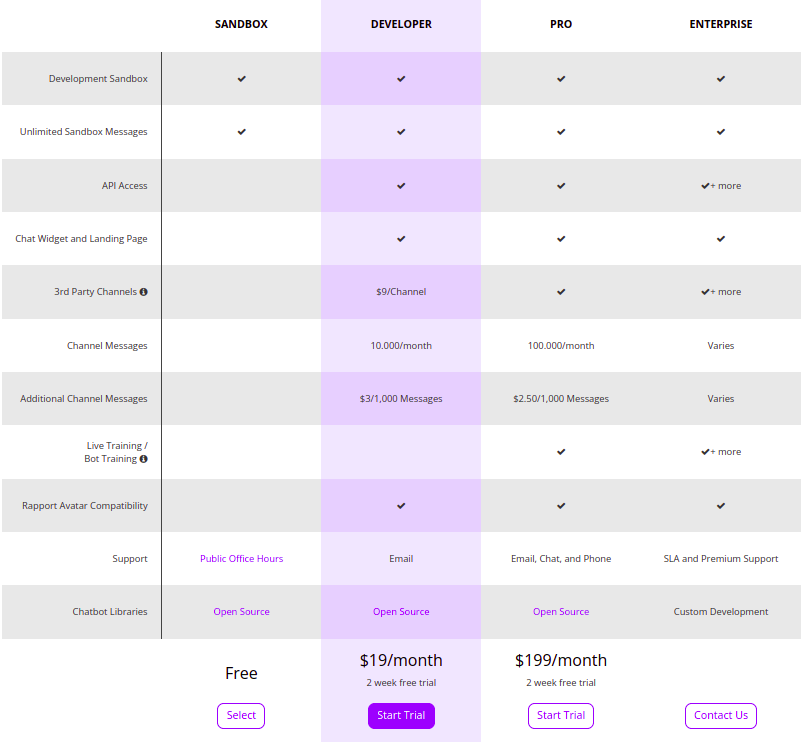
\includegraphics[width=1.0\textwidth]{imagenes/02_EstadoDelArte/cuentas_pandorabots.png}
\begin{center}
Fuente: \url{https://developer.pandorabots.com/home.html}
\end{center}
\caption{Cuentas disponibles en Pandorabots}
\label{fig:cuenta_pandorabots}
\end{figure}

En la Figura \ref{fig:cuenta_pandorabots} podemos comprobar como con la cuenta gratuita no disponemos de todas las funcionalidades anteriormente descritas.

\subsubsection*{Extensibilidad}

Dado que hay muchos \glspl{framework} para la creación de un chatbot con AIML, dependerá del \gls{framework} elegido la cantidad de posibilidades de conexiones con \glspl{API} o servicios externos al chatbot.

Para que AIML sea flexible y extensible dispone de la posibilidad de integrar sus propias \glspl{API}, bases de datos o también se pueden crear etiquetas propias; pero para ello se debe tener cierto nivel con el lenguaje de programación AIML.

Si optamos por servicios web como Pandorabots para poder disponer de conexión con servicios externos al servicio web o con \glspl{API} se debe disponer de una cuenta de pago, no basta con la versión gratuita de Pandorabots.

\subsubsection*{Integración}

Si optamos por servicios web como Pandorabots, al igual que pasa con la extensibilidad, será necesaria una cuenta de pago para poder integrar nuestro chatbot en plataformas de mensajería como Facebook Messenger, Twitter, Telegram y muchos más.

Pero si optamos por \glspl{framework} de código abierto, hay una multitud de posibilidades, tantas como el nivel de conocimientos que tenga el creador del chatbot. Un ejemplo puede ser con Node JS, donde podríamos desplegar el chatbot en cualquier página web a través de una interfaz web que enviase peticiones al servidor creado con Node JS que aloja al chatbot.

\subsubsection*{Ejemplos}

Algunos ejemplos de chatbot implementados con AIML son los siguientes:

\begin{itemize}
\item \textbf{Rosie}. Chatbot base basado en ALICE 2.0 \footnote{\url{https://github.com/pandorabots/rosie}}
\item \textbf{Cathy}. Chatbot para Discord basado en Python 3 y AIML \footnote{\url{https://github.com/DevDungeon/Cathy}}
\end{itemize}


\subsection{IBM Watson}

\subsubsection*{Información general}

IBM Watson es un \gls{portfolio} de IBM de aplicaciones, herramientas y soluciones preparadas para la empresa, diseñado para reducir los costes y los obstáculos de \gls{IA}, además de optimizar los resultados y el uso responsable de la \gls{IA} según se indica en su página oficial \cite{RefWorks:RefID:15-2021ibm}. Aunque en un inicio IBM Watson no era lo que es actualmente y tampoco se buscaba llegar a este punto. Originalmente, IBM Watson surgió como el siguiente gran desafío de la empresa IBM, tras haber salido victorioso de otros grandes desafíos como la victoria de Deep Blue contra Garry Kasparov y el desafío de la supercomputadora Blue Gene. El objetivo que perseguía en sus orígenes Watson era conseguir ganar a competidores humanos en el concurso Jeopardy. Este concurso de televisión estadounidense consistía en un concurso de preguntas sobre una multitud de temas, y los concursantes deberán resolver las preguntas de cada prueba realizando preguntas sobre las pistas que va dando el presentador. Las reglas del concurso obligan a que Watson no únicamente sepa conocimientos sobre los temas que se utilizan en el concurso, sino también a saber efectuar preguntas al presentador basándose en sus pistas, y además saber distinguir cuando la pista del presentador no es cierta. Todos estos requisitos convierten el ganar este concurso en un gran desafío, la empresa IBM se embarcó en este proyecto a mediados de la década del 2000. Finalmente, en el año 2011 se llegó a un acuerdo para la realización del programa, donde compitieron dos grandes ex-concursantes del programa como son Ken Jennings y Brad Rutter contra Watson. Tal y como se indica en el artículo \cite{RefWorks:RefID:16-best2013ibm}, Watson ganó el juego con \$77.147, dejando a Rutter y Jennings con \$21.600 y \$24.000 respectivamente.

Tras la victoria de IBM Watson, se empezó a enfocar y rediseñar a Watson hacia distintos sectores como la medicina, la banca o los agentes conversacionales, entre otras. Los agentes conversacionales es el sector que nos interesa investigar.

Dado que IBM Watson está orientado al mundo empresarial, destaca por su confianza, es decir, Watson es transparente en cuanto a las decisiones basadas en \gls{IA}; también protege la privacidad de los datos y su seguridad. Todas estas características son muy valoradas en cualquier producto empresarial, incluso algunas son imprescindibles.

Otra característica de Watson es su procesamiento del lenguaje natural. Al igual que AIML es multilenguaje, pero Watson lo lleva a un aspecto más complejo, añadiendo la capacidad de analizar datos complejos y no estructurados, como pueden ser códigos de programación o incluso formas de expresión específicas de una modalidad de trabajo. Este procesamiento del lenguaje natural no es algo alcanzable por cualquier empresa. La \gls{IA} de Watson sabe desenvolverse en las situaciones más complejas, como pueden ser situaciones en las que no pueda responder, reenviando la solicitud a un agente humano o hacia algún documento de ayuda; evitando realizar preguntas redundantes facilitando la comunicación y haciéndola más natural; y por último sabe manejar solicitudes ambiguas que son comunes en la comunicación como pueden ser errores ortográficos, cambios de tema, y muchas más situaciones que pueden ser inesperadas para el chatbot en una conversación. Además, IBM Watson intenta mejorar su rendimiento aportando al creador del chatbot información sobre que nuevos temas añadir para mejorar la respuesta a las solicitudes.

Y por último, destaca que Watson trabaja con cualquier servicio en la nube, lo que facilita su integración en las empresas, ya que no será un impedimento el lugar donde residan los datos de la empresa. Y además el trabajar en \gls{cloud} facilitará el trabajo con los datos.

En concreto, en la página oficial de IBM Watson Assistant \cite{RefWorks:RefID:17-ibm} se destaca la rentabilidad del producto, de hasta un 337\% según el Informe TEI de Forrester \cite{RefWorks:RefID:8-iles2020el}; su precisión, de hasta un 14,7\% superior que las soluciones de la competencia según un reciente estudio publicado sobre machine learning \cite{RefWorks:RefID:18-2020watson}; y su fiabilidad, ya que Watson tiene más de 1000 despliegues de clientes en todos los sectores.

\subsubsection*{Uso}

IBM Watson está pensado para ser utilizado por cualquier persona, da igual que no tenga conocimientos en programación. La creación del chatbot se basa en un editor de arrastrar y soltar. Este editor evita la complejidad de la programación de un chatbot y los posibles errores derivados de esa necesidad de escribir el código en su creación o en alguna modificación que necesite el chatbot. Es posible crear un chatbot sin escribir una sola línea de código.

\begin{figure}[h]
\centering
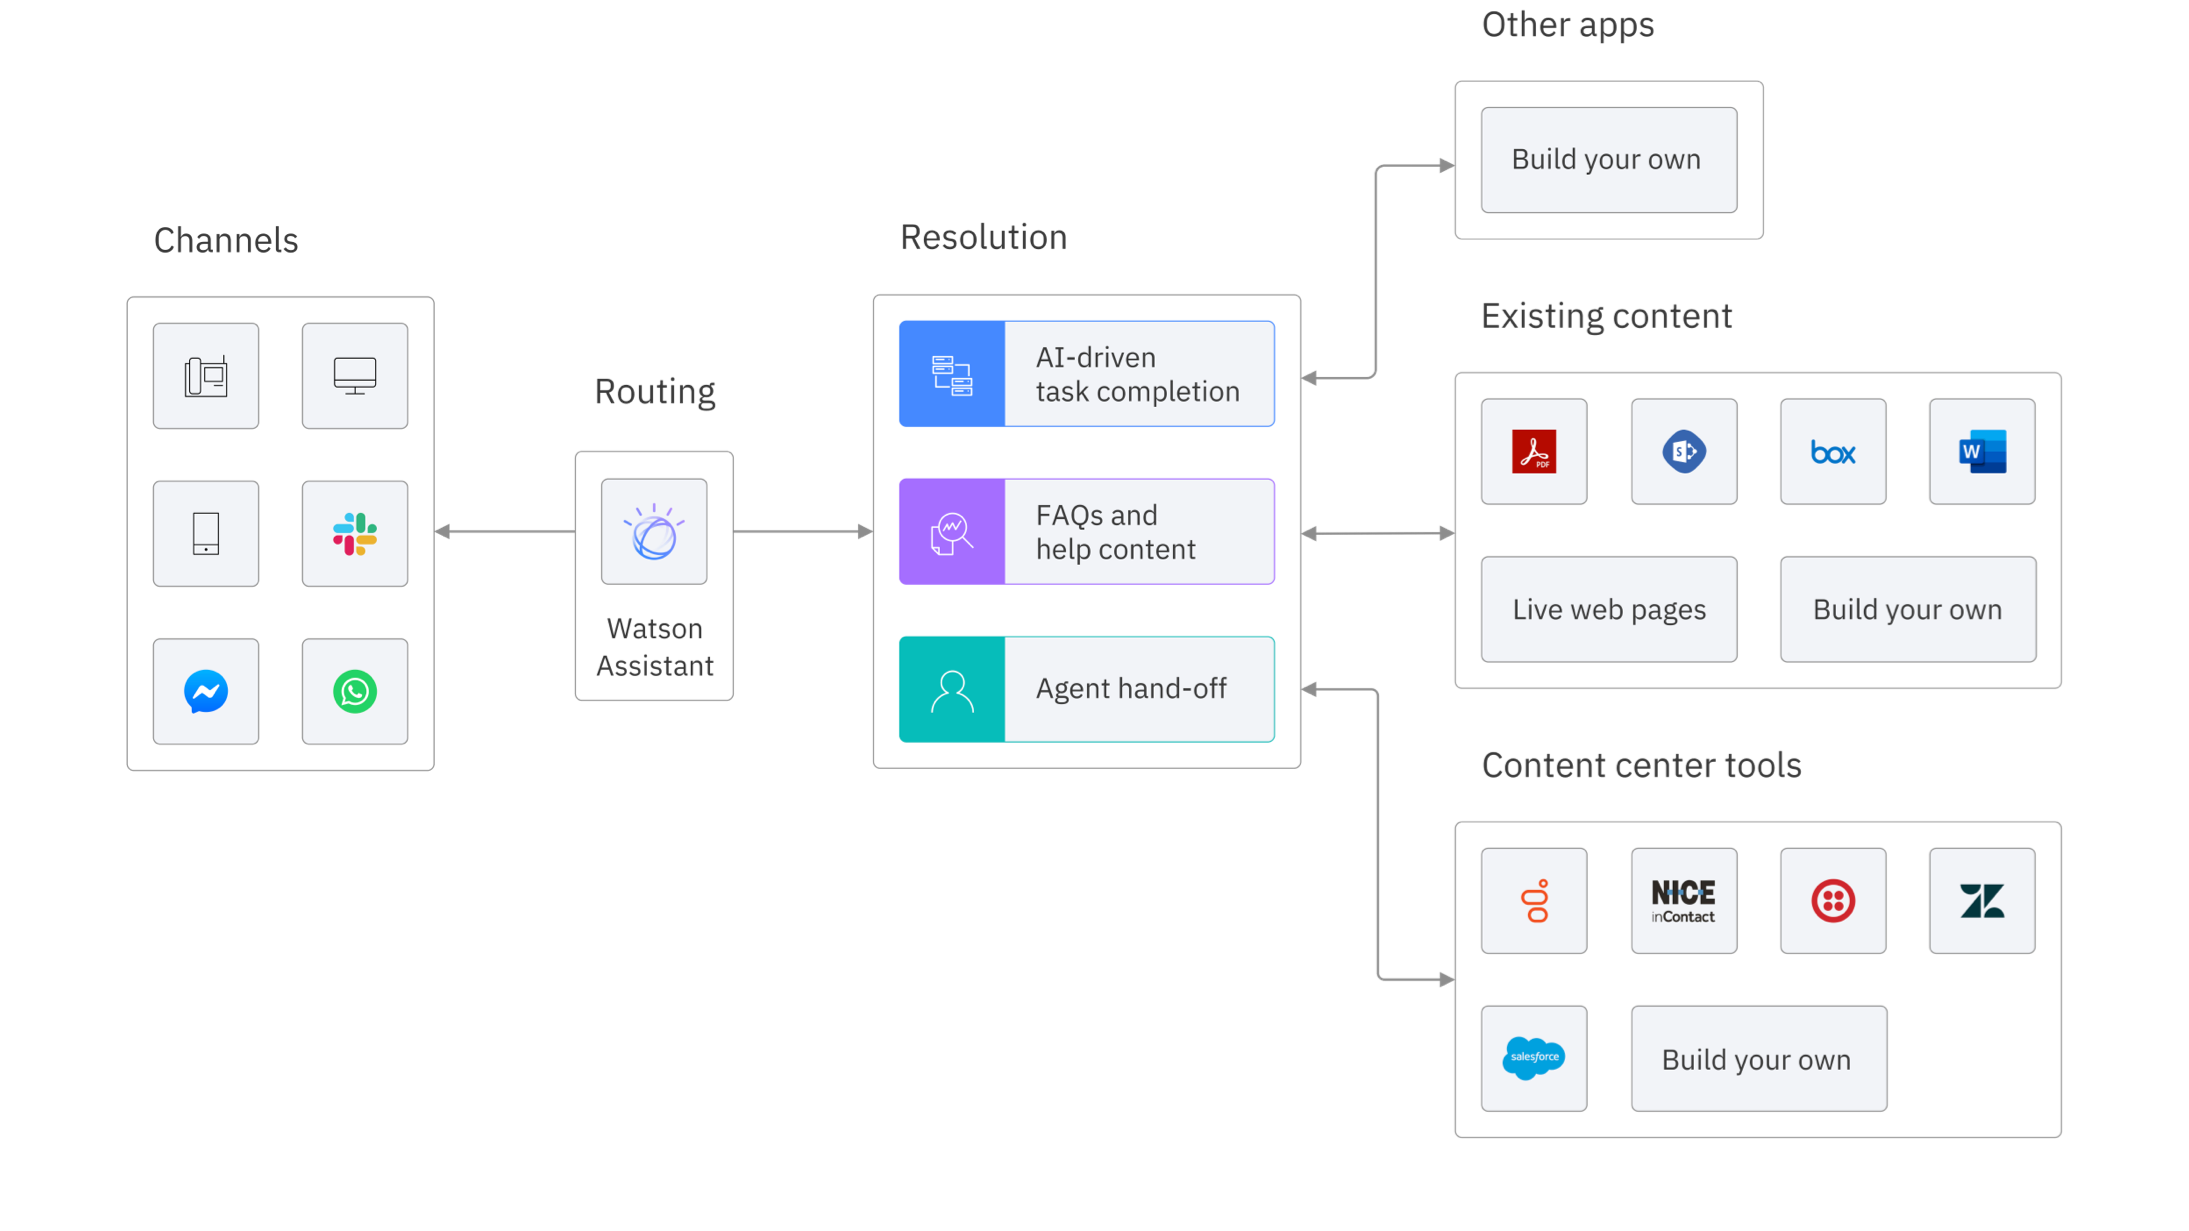
\includegraphics[width=1.0\textwidth]{imagenes/02_EstadoDelArte/editor_IBM_Watson.png}
\begin{center}
Fuente: \url{https://www.ibm.com/es-es/products/watson-assistant}
\end{center}
\caption{Editor de IBM Watson}
\end{figure}

La IA del chatbot es capaz de comprender un tema en cualquier lenguaje natural con unas pocas frases, facilitando la adaptación del chatbot a la funcionalidad que se le quiera dar, adaptándose de forma rápida y precisa al dominio del proyecto.

\subsubsection*{Extensibilidad}

Como se ha indicado en apartados anteriores, IBM Watson es un \gls{portfolio} de IBM de aplicaciones. En su página oficial \cite{RefWorks:RefID:19-2021productos} se indican las siguientes aplicaciones con las que se puede integrar el chatbot:

\begin{itemize}
\item IBM Watson Discovery
\item IBM Watson Natural Language Understanding
\item IBM Watson Speech to Text
\item IBM Watson Text to Speech
\item IBM Watson Knowledge Studio
\item IBM Watson Language Translator
\item IBM Watson Natural Language Classifier
\end{itemize}

Entre estas aplicaciones se encuentran algunas muy útiles como IBM Watson Discovery para la extracción y búsqueda de información, IBM Watson Speech to Text para transformar la voz a texto escrito gracias a una potente tecnología de machine learning, IBM Watson Language Translator para traducir dinámicamente información, o IBM Watson Knowledge Studio para enseñar a Watson el idioma del dominio del chatbot.

\subsubsection*{Integración}

El chatbot se puede integrar como un chat web, como contestador de llamadas de teléfono o como un chatbot en una aplicación de mensajería como WhatsApp, Facebook Messenger, SMS y muchos más. Todas estas maneras de integrar el chatbot son muy fáciles de realizar.

\subsubsection*{Ejemplos}

Algunos ejemplos de chatbot implementados con Watson son los siguientes:

\begin{itemize}
\item \textbf{Nanci. Chatbot desarrollado por la empresa GM Financial} \footnote{\url{https://www.gmfinancial.com/en-us/company/newsroom/chatbot.html}}
\item \textbf{Chatbot desarrollado por la empresa Bradesco} \footnote{\url{https://www.ibm.com/watson/stories/bradesco}}
\item \textbf{CARL. Chatbot desarrollado por la empresa Siemens} \footnote{\url{https://www.ibm.com/es-es/products/watson-assistant/client-stories}}
\item \textbf{Chatbot desarrollado por la empresa Humana} \footnote{\url{https://www.ibm.com/watson/stories/humana}}
\end{itemize}


\subsection{Google Dialogflow}\label{subsec:dialogflow}

\subsubsection*{Información general}

Dialogflow pertenece a la empresa Google, aunque no fue desarrollada originalmente por ella. Google adquirió API.AI en el año 2016 y le cambió el nombre a Dialogflow. Desde su adquisición, Google ha mejorado Dialogflow gracias a sus técnicas de \gls{IA} de gran calidad. Esta plataforma es una de las más utilizadas para la creación de chatbots junto con IBM Watson, aunque a diferencia de Watson, Dialogflow está enfocado tanto para el mundo empresarial como para usuarios particulares que están empezando en el mundo de los chatbots. Esta variedad en la complejidad del chatbot es posible gracias a una interfaz que permite crear un chatbot con unos mínimos conocimientos técnicos, únicamente será necesario introducir las frases de las preguntas y de las respuestas para construir el chatbot. Y si se quiere generar un chatbot más complejo, podemos introducirnos en la configuración del chatbot o integrar más funcionalidades que aumenten su complejidad.

Dentro de Dialogflow existen dos tipos de agentes, los Agentes de ES y los agentes de CX. Dentro de los agentes de ES existen dos ediciones, la edición de prueba y la edición Essentials. Con la versión de prueba no se puede acceder a los servicios de Google Cloud, pero las entradas y salidas son gratuitas; mientras que con la versión Essentials si se puede acceder a esos servicios, pero las entradas y salidas del agente empezarán a costar dinero. Entre la versión Essentials y la versión CX la principal diferencia es que en la versión CX la relación entre los intents se define mediante un diagrama de flujo, mientras que en la versión Essential la relación entre los intents se define mediante los contextos. La limitación de los contextos es que no posibilitan la relación de varios intents con otro intent. La versión CX ha sido lanzada hace unos pocos meses, por lo que es algo novedosa y es útil para aquellos que quieran realizar un chatbot algo más complejo o que ya tengan experiencia con la plataforma. La versión Essentials está más enfocada a agentes de complejidad media y la versión CX está más enfocada a agentes de complejidad alta. Aunque la curva de aprendizaje es más suave en la edición CX, la edición CX no dispone actualmente de todas las funcionalidades presentes en la edición Essentials.

\subsubsection*{Uso}

Para empezar a crear un chatbot con Dialogflow será necesaria una cuenta Google. Los apartados claves para la creación de un bot son Intents y Entities.

Dentro del apartado Intents se generan los distintos intents a usar en el chatbot, cada intent es un estado al que accede el chatbot si se cumple el contexto y se detecta una de las frases de entrenamiento del intent. Los contextos sirven para guardar información adquirida que puede resultar útil durante la conversación, como el nombre del usuario que está utilizando el chatbot; además de la información que se quiere conservar, también se puede indicar durante cuento tiempo se estima que es útil esa información, también llamado lifespan. Dentro de cada intent se debe también definir las posibles respuestas que envía el chatbot si se activa el intent. Y por último a cada intent se le pueden añadir eventos. Por defecto, en el apartado Intents vienen creados los siguientes intents:

\begin{itemize}
\item Default Fallback Intent: Intent para cuándo el chatbot no reconoce la pregunta
\item Default Welcome Intent: Intent para dar la bienvenida al chatbot
\end{itemize}

Dentro del apartado Entities se generan las distintas entidades. Una entidad es un conjunto de ejemplos sobre un tema, por ejemplo, la entidad países contiene los siguientes elementos: España, Francia, Italia, etc. Cuando se define una entidad se deben indicar los elementos que la forman, pero adicionalmente se puede indicar los sinónimos de los elementos, este añadido le dará una mayor naturalidad a la conversación al hacer que los textos no sean tan estáticos.

Otro apartado importante para el desarrollo del chatbot es el apartado Training, donde se podrán analizar las conversaciones que se han realizado con el chatbot e indicar si se ha respondido adecuadamente o no, esta acción de aceptación o no hará que el chatbot sea más preciso con sus respuestas. Si se acepta una respuesta, si la pregunta hecha por el usuario no se encuentra entre las preguntas del intent activado, se añade a la lista de preguntas del intent.

\subsubsection*{Extensibilidad}

Dialogflow permite integrar un \gls{webhook}. Este \gls{webhook} puede estar alojado tanto en un servidor externo como en Google Cloud. Si se opta por la opción de Google Cloud, para lo que es necesario una cuenta Google de pago, se pueden añadir los archivos que componen el \gls{webhook} en el apartado Fulfillment dentro de un editor en línea. Si se opta por la opción de un servidor externo, tanto si es local como si es en una plataforma en la nube, se deberá añadir la URL del servidor web en el mismo apartado que se indicó anteriormente. La conexión con el servidor externo se realizará mediante el envío de peticiones tipo POST. Estas peticiones contendrán la información en formato JSON. Para que la información se envíe al servidor, independientemente de la opción que se elija, se debe activar en los intents elegidos la opción del \gls{webhook}, de esta forma cuando se active el intent se enviará una petición al servidor web.

Una vez se tenga una conexión con un servidor web, dentro de este servidor se podrán añadir más funcionalidad, como BBDD o interpretes de AIML, que permitirán seguir extendiendo el chatbot.

\subsubsection*{Integración}

El chatbot se puede integrar en canales de telefonía, como Twilio; en canales de mensajería, como Telegram, Facebook Messenger o Twitter; en canales de videollamadas, como Skype; y en páginas web a modo de chat web.

\subsubsection*{Ejemplos}

Algunos ejemplos de chatbot implementados con Dialogflow son los siguientes:

\begin{itemize}
\item \textbf{SAM. Chatbot desarrollado por la empresa Ubisoft} \footnote{\url{https://www.hd-tecnologia.com/ubisoft-ia-personal-sam-primer-asistente-gaming}}
\item \textbf{Chatbot desarrollado por la empresa Dominos Pizza} \footnote{Caso de estudio de Dominos Pizza \cite{RefWorks:RefID:10-domino's-case-study}}
\item \textbf{Chatbot desarrollado por la empresa Malaysia Airlines} \footnote{\url{https://cloud.google.com/customers/malaysia-airlines}}
\end{itemize}


\subsection{Rasa Stack}

\subsubsection*{Información general}

Rasa Stack es un conjunto de herramientas de aprendizaje automático de código abierto para el desarrollo de chatbots. Rasa Stack está desarrollado por una comunidad de personas pertenecientes a muchos lugares del mundo, de modo que esta plataforma, a diferencia de las dos anteriores, no está respaldada por ninguna de las grandes empresas tecnológicas como pueden ser Google o IBM. Pero esto no quiere decir que no sea una buena plataforma, ya que ha sido probada por grandes empresas como AIRBUS, TOYOTA o Adobe.

En su página oficial \cite{RefWorks:RefID:20-2020rasa} se destaca la gran personalización que pueden alcanzar los chatbots en esta plataforma.

Dentro de Rasa Stack se pueden distinguir dos tipos de cuenta, la cuenta para empresas (Rasa Enterprise) y la cuenta gratuita (Rasa Open Source o Rasa X). La diferencia entre Rasa Open Source y Rasa X es que Rasa X no es de código abierto, mientras que Rasa Open Source, como indica su nombre, si es de código abierto. La cuenta para empresas proporciona funcionalidades muy útiles para productos empresariales como pueden ser realizar análisis del chatbot, acceso con roles a la plataforma, disponibilidad de un soporte de calidad, y mucho más.

En Rasa Stack se destaca que los chatbots creados en esta plataforma no se convierten en \glspl{caja_negra}, sino que el funcionamiento del chatbot es transparente, por lo tanto, se tiene total acceso a la configuración de todo el chatbot, incluido el modelo usado en el entrenamiento del bot.

\subsubsection*{Uso}

Al igual que pasa en Dialogflow, Rasa Stack mantiene un contexto de la conversación, donde se guarda información proporcionada por el usuario, lo que permite una conversación más natural al no hacer preguntas redundantes.

La creación del chatbot se divide en dos módulos, Rasa NLU y Rasa Core. La plataforma proporciona unas \gls{NLU}, estas \gls{NLU} se pueden entrenar sobre la base de una lista de mensajes, a cada mensaje se le asignará una intención y las entidades que contiene. Una vez está entrenado el módulo \gls{NLU}, se procede a configurar el módulo Rasa Core, que es el encargado de confeccionar la respuesta del chatbot a la pregunta identificada por el módulo Rasa NLU. La configuración de Rasa Core consiste en escribir las respuestas de los distintos intents, definir el dominio del chatbot, definir la conexiones con \glspl{API}, y definir el modelo de gestión del diálogo, por ejemplo, una \gls{CNN}, citando además las políticas que se van a usar.

\subsubsection*{Extensibilidad}

La transparencia que tienen los chatbots permiten conectar con él muchas \glspl{API} externas que suman más funcionalidades aparte de las que ya proporciona la plataforma. Y al igual que pasa con Dialogflow, se puede conectar a un servidor web y a este servidor conectar las \glspl{API}.

\subsubsection*{Integración}

Tal y como se indica en su página oficial \cite{RefWorks:RefID:20-2020rasa}, un chatbot creado con Rasa Stack se puede integrar en canales como IVR, chat y SMS. Además, se indica que Rasa Stack admite 10 canales de mensajería integrados, como pueden ser Telegram, Facebook Messenger, Slack y algunos más; y que adicionalmente proporciona un punto de conexión con cualquier plataforma de comunicación, como puede ser un servidor web.

\subsubsection*{Ejemplos}

Algunos ejemplos de chatbot implementados con Rasa Stack son los siguientes:

\begin{itemize}
\item \textbf{Djingo. Chatbot desarrollado por la empresa Orange} \footnote{\url{https://rasa.com/customers/orange}}
\item \textbf{Chatbot desarrollado por la empresa TMobile} \footnote{\url{https://rasa.com/customers/t-mobile}}
\item \textbf{Chatbot desarrollado por la empresa Helvetia} \footnote{\url{https://rasa.com/customers/helvetia}}
\end{itemize}


\subsection{GPT-3}

\subsubsection*{Información general}

GPT-3 (Generative Pre-trained Transformer 3) es un conjunto de modelos de \gls{IA} desarrollados por la empresa OpenAI en el año 2020. Este modelo es la tercera generación de estos modelos de inteligencia artificial. En concreto, este último modelo tiene 175 billones de parámetros, lo cual es una potencia impresionante que le permite generar texto que parece escrito por humanos y no por máquinas, es incluso capaz de escribir código. GPT-3 se ha visto potenciado por la inversión de Microsoft entre otros. Este modelo ha revolucionado el procesamiento y la generación de lenguaje natural. Esta última generación es de pago, cobrando cada cierta cantidad de tokens analizados, en concreto cada 1000 tokens actualmente, según se indica en su página de precios \cite{RefWorks:RefID:21-openai.}. Un token es un conjunto de palabras o un conjunto de letras, su tamaño depende también del lenguaje que se esté usando. Si se quiere saber más sobre los tokens se puede emplear la herramienta Tokenizer \footnote{\url{https://beta.openai.com/tokenizer}}, que nos proporciona OpenAI, para calcular el número de tokens en una frase. Algo importante es que únicamente se paga por lo que se emplea, no como en otras páginas que independientemente de lo que se emplee un servicio se paga una cuota fija.

Como se ha indicado anteriormente, GPT-3 es un conjunto de modelos. Según se indica en su página web \cite{RefWorks:RefID:22-modelos} existen los siguientes modelos:

\begin{itemize}
\item Davinci
\item Curie
\item Babbage
\item Ada
\end{itemize}

La diferencia entre los distintos modelos son su potencia, velocidad y coste por token. El modelo Davinci es el más potente y el más caro, mientras que el modelo Ada es el más rápido y barato.

Las posibles aplicaciones de GPT-3, según su página de ejemplos \cite{RefWorks:RefID:23-openai.}, son las siguientes:

\begin{itemize}
\item Generación de lenguaje natural
\item Clasificación
\item Generación de código
\item Chatbot
\item Traducción (tanto código como lenguaje natural)
\end{itemize}

La aplicación de GPT-3 como un chatbot se explicará más en detalle en el siguiente apartado.

Un problema de GPT-3 es que se trata de una herramienta muy cara, ya que necesita una enorme cantidad de potencia informática para funcionar, por lo tanto, su uso se limita solamente a empresas.

\subsubsection*{Uso}

Dado que GPT-3 es un modelo de aprendizaje, no es una plataforma como las vistas hasta el momento, para poder crear un chatbot será necesario hacer uso de un lenguaje de programación como Python para elaborar el chatbot. En la sección de bibliotecas de OpenAI \footnote{https://beta.openai.com/docs/libraries/libraries} se pueden encontrar todas las bibliotecas, tanto oficiales como de la comunidad, para poder emplear GPT-3 con distintos lenguajes de programación.

El chatbot consistirá en sucesivas llamadas a la \gls{API} de OpenAI para obtener las respuestas del chatbot. A continuación se puede observar el código en Python necesario para realizar una llamada a la \gls{API}:

\begin{lstlisting}
import openai

openai.Completion.create(
engine="davinci",
prompt="Make a list of astronomical observatories:"
)
\end{lstlisting}
\begin{center}
Fuente: \url{https://openai.com/api}
\end{center}
\begin{center}
\caption{Ejemplo de llamada a la API de OpenAI}
\end{center}

También se puede hacer empleo del Playground \footnote{https://beta.openai.com/playground} de OpenAI para utilizar las distintas funcionalidades de GPT-3.

GPT-3 ha sido entrenado con millones de datos, pero dispone de una herramienta para enfocar su modelo a los datos que vayamos a usar en nuestro chatbot. Esta herramienta es el fine-tuning, que consiste en seguir entrenando el modelo con un conjunto de datos durante un cierto número de \gls{epocas}, a elección del creador del chatbot, permitiendo generar textos relacionados con el dominio del chatbot.

Los datos del conjunto de entrenamiento deberán ser formateados de cierta forma para poder entrenar con ellos. Para formatear los datos, OpenAI dispone de una herramienta que lo posibilita. Al igual que para inferir textos con GPT-3 es necesario pagar cada cierta cantidad de tokens, pasa lo mismo con el fine-tuning de los modelos. En la documentación \cite{RefWorks:RefID:25-openai.} se indica el precio de entrenar los distintos modelos.

Una vez se tenga el modelo listo, algo que hay que tener en cuenta durante la creación del chatbot es el mantenimiento de un contexto durante las conversaciones, ya que con GPT-3 cada vez que se llama a la \gls{API} no se dispone de un contexto, cosa que por ejemplo si se tenía en Dialogflow, únicamente se dispone de la información que se le pase con la llamada.

Una solución a este problema podría ser la creación de una base de datos, por ejemplo con PostgreSQL que dispone de un tipo muy útil para los textos. Con esta base de datos se irá guardando información de las anteriores preguntas, la cual se le pasará al modelo junto con la pregunta a realizar.

\subsubsection*{Extensibilidad}

En la página oficial no se hace referencia a ninguna funcionalidad externa, pero el hecho de que se puedan hacer llamadas a la \gls{API} con distintos lenguajes de programación, permite que todas las funcionalidades de las que dispongan estos lenguajes se puedan usar junto con GPT-3.

\subsubsection*{Integración}

La integración no es tan sencilla como podría ser en plataformas como Dialogflow, dado que en la creación del chatbot con GPT-3 solamente se implementa el \gls{back-end} del chatbot, por lo tanto, se deberá implementar, por parte del creador del chatbot, el \gls{front-end} del mismo. Para implementar el \gls{front-end} se dispone de muchas posibilidades, como podría ser implementar un chat web o una APP, entre otras.

\subsubsection*{Ejemplos}

Algunos ejemplos de chatbot implementados con GPT-3 son los siguientes:

\begin{itemize}
\item \textbf{Chatbot para Telegram} \footnote{https://github.com/xwarfare/GPT3-Telegram-Chatbot}
\item \textbf{Chatbot para WhatsApp} \footnote{https://github.com/theshanergy/whatbot}
\item \textbf{Marcus. Chatbot para guía de viajes} \footnote{https://github.com/manan-paneri-99/marcus-gpt3-bot}
\end{itemize}


\subsection{BlenderBot}

\subsubsection*{Información general}

BlenderBot es un proyecto de código abierto desarrollado por la empresa Facebook. En este trabajo vamos a analizar la versión 1 de este chatbot, ya que recientemente se ha lanzado su segunda versión. Se trata de uno de los chatbots de código abierto con mayor dominio. Y como indica Facebook \cite{RefWorks:RefID:41-roller2020recipes}, además, durante una conversación este chatbot es capaz de generar una sensación de humanidad que pocos chatbots pueden igualar. Una característica de este chatbot, el cual fue el primero en poseerla, que está relacionada con su nombre, es su mezcla de habilidades conversacionales, como pueden ser la empatía, el conocimiento y la personalidad en un solo sistema. Este chatbot tiene distintas configuraciones, las cuales se diferencian por su número de parámetros o dicho de otra manera por su potencia.

BlenderBot mejoró la potencia de los chatbots anteriores a él, sin perder la eficiencia necesaria para entablar una conversación de forma fluida. Esta mejora fue posible gracias a las distintas técnicas usadas por Facebook \cite{RefWorks:RefID:41-roller2020recipes}, como son el paralelismo de modelos por columna o la división de la red neuronal en partes más pequeñas y manejables.

Otro punto importante en los chatbots es el conjunto de entrenamiento empleado, ya que el chatbot imitará todos los comportamientos de las frases de los conjuntos, tanto buenas como malas, heredando todos los sesgos del conjunto. BlenderBot introdujo una novedosa tarea llamada Blended Skill Talk (BST). Como se indica en el artículo de Facebook \cite{RefWorks:RefID:41-roller2020recipes}, estas tareas consiste en las siguientes habilidades asociadas con su respectivo conjunto de entrenamiento:

\begin{itemize}
\item Uso atractivo de la personalidad (PersonaChat)
\item Uso atractivo del conocimiento (Wizard of Wikipedia)
\item Muestra de empatía (Empathetic Dialogues)
\item Capacidad para combinar los tres a la perfección (BST)
\end{itemize}

La combinación de estas habilidades es un desafío difícil porque los sistemas deben poder cambiar entre diferentes tareas cuando sea apropiado, como ajustar el tono si una persona cambia de broma a seria. Nuestro nuevo conjunto de datos BST proporciona una manera de crear sistemas que combinen y muestren estos comportamientos.

\subsubsection*{Uso}

De igual modo que pasa con GPT-3, esta herramienta para generar un chatbot necesitará de un lenguaje de programación, dado que la herramienta únicamente consiste en un modelo de aprendizaje. El chatbot consistirá en sucesivas inferencias del modelo para obtener las respuestas del chatbot.

\subsubsection*{Extensibilidad}

En este apartado paso lo mismo que en el anterior apartado. El chatbot dispone de todas las funcionalidades de las que disponen los lenguajes usados para generar el chatbot.

\subsubsection*{Integración}

En la creación del chatbot con BlenderBot solo se implementa el \gls{back-end} del chatbot, por lo tanto, se deberá implementar, por parte del creador del chatbot, el \gls{front-end} del mismo. Para implementar el \gls{front-end} se dispone de muchas posibilidades, como podría ser implementar un chat web o una APP, entre otras.




\section{Comparativa de las herramientas}

Después de revisar las distintas herramientas, es hora de compararlas para facilitar la elección de una ellas para el desarrollo del proyecto. En primer lugar, se hará una comparación de pros y contras de todas las herramientas (Tabla \ref{tab:pros_contras_plataformas}), y seguidamente se mostrará una tabla (Tabla \ref{tab:carac_plataformas}) con una serie de características, indicando cuáles están presentes en las distintas herramientas.


\begin{table}[h]
\centering
\resizebox{\textwidth}{!}{%
\begin{tabular}{c|l|l|}
\cline{2-3}
\multicolumn{1}{l|}{} &
  \multicolumn{1}{c|}{\cellcolor[HTML]{FFFC9E}\textbf{PROS}} &
  \multicolumn{1}{c|}{\cellcolor[HTML]{FFFC9E}\textbf{CONTRAS}} \\ \hline
\multicolumn{1}{|c|}{\cellcolor[HTML]{FFCCC9}\textbf{AIML}} &
  \begin{tabular}[c]{@{}l@{}}- Multilenguaje\\ - El chatbot no es un caja negra\\ - Lenguaje de programación simple\\ - Posibilidad de conexión con APIs propias\\ - Muchas funcionalidades de forma gratuita\end{tabular} &
  \begin{tabular}[c]{@{}l@{}}- Alto gasto de tiempo en la creación del agente conversacional\\ - Necesidad de una cuenta de pago usando servicios web\\ - No es una plataforma en la nube\\ - Conversaciones poco naturales y poco flexibles\end{tabular} \\ \hline
\multicolumn{1}{|c|}{\cellcolor[HTML]{FFCCC9}\textbf{IBM Watson}} &
  \begin{tabular}[c]{@{}l@{}}- Posibilidad de crear chatbots muy complejos\\ - Gran cantidad de conexiones con APIs de mucha calidad\\ - Editor de arratrar y soltar\\ - Facilidad de desplegar el chatbot en muchos canales importantes\\ - Es una plataforma en la nube\end{tabular} &
  \begin{tabular}[c]{@{}l@{}}- Necesidad de una cuenta de pago para crear chatbot complejos\\ - Enfocado para el mundo empresarial\\ - El chatbot es una caja negra\end{tabular} \\ \hline
\multicolumn{1}{|c|}{\cellcolor[HTML]{FFCCC9}\textbf{Dialogflow}} &
  \begin{tabular}[c]{@{}l@{}}- Posibilidad de crear chatbots muy complejos sin necesidad de pago\\ - Posibilidad de conexión con un servidor web de forma gratuita\\ - Facilidad de desplegar el chatbot en muchos canales importantes\\ - Creación de chatbots usando sólo frases y entidades\\ - Es una plataforma en la nube\end{tabular} &
  \begin{tabular}[c]{@{}l@{}}- Para hacer agentes muy complejos es necesario gastar tiempo \\ en la creación del servidor\\ - Se necesita tener cierto conocimiento de la plataforma para \\ sacar todo su potencial\\ - Calidad regular en la documentación\\ - Parte del chatbot es una caja negra\end{tabular} \\ \hline
\multicolumn{1}{|c|}{\cellcolor[HTML]{FFCCC9}\textbf{Rasa Stack}} &
  \begin{tabular}[c]{@{}l@{}}- Documentación de calidad\\ - El chatbot no es un caja negra\\ - Facilidad de desplegar el chatbot en muchos canales importantes\\ - Posibilidad de crear chatbots muy complejos\end{tabular} &
  \begin{tabular}[c]{@{}l@{}}- Necesidad de alto nivel técnico\\ - Plataforma en desarrollo\\ - Necesidad de mucho tiempo para la creación del chatbot\\ - No es una plataforma en la nube\end{tabular} \\ \hline
\multicolumn{1}{|c|}{\cellcolor[HTML]{FFCCC9}\textbf{GPT-3}} &
  \begin{tabular}[c]{@{}l@{}}- Posibilidad de crear chatbots muy complejos\\ - Chatbots con una conversación muy natural\\ - Buena documentación\end{tabular} &
  \begin{tabular}[c]{@{}l@{}}- Necesidad de conocimientos técnicos\\ - Necesidad de pago para hacer uso de los servicios\\ - Necesidad de una solución para mantener el contexto\\ - Requiere de un conjunto de datos para poder adaptar el \\ chatbot a su dominio\\ - Requiere de una plataforma a parte para el despliegue\end{tabular} \\ \hline
\multicolumn{1}{|c|}{\cellcolor[HTML]{FFCCC9}\textbf{BlenderBot}} &
  \begin{tabular}[c]{@{}l@{}}- Posibilidad de crear chatbots muy complejos\\ - Chatbots con una conversación muy natural\\ - Uso gratuito\\ - Buena documentación\end{tabular} &
  \begin{tabular}[c]{@{}l@{}}- Necesidad de conocimientos técnicos\\ - Necesidad de una solución para mantener el contexto\\ - Requiere de un conjunto de datos para poder adaptar el \\ chatbot a su dominio\\ - Requiere de una plataforma a parte para el despliegue\end{tabular} \\ \hline
\end{tabular}%
}
\caption{Comparativa de pros y contras de las herramientas de desarrollo}
\label{tab:pros_contras_plataformas}
\end{table}


\begin{table}[h]
\centering
\resizebox{\textwidth}{!}{%
\begin{tabular}{|c|c|c|c|c|c|c|c|c|}
\hline
\rowcolor[HTML]{FFFC9E} 
\textbf{Nombre} &
  \textbf{Código abierto} &
  \textbf{Multilenguaje} &
  \textbf{\begin{tabular}[c]{@{}c@{}}Necesidad \\ Conocimientos técnicos\end{tabular}} &
  \textbf{Cloud Service} &
  \textbf{\begin{tabular}[c]{@{}c@{}}Elaboración de\\ Chatbot complejos\\ con facilidad\end{tabular}} &
  \textbf{\begin{tabular}[c]{@{}c@{}}Conversación con\\ naturalidad\end{tabular}} &
  \textbf{\begin{tabular}[c]{@{}c@{}}Documentación \\ de gran\\  calidad\end{tabular}} &
  \textbf{\begin{tabular}[c]{@{}c@{}}Facilidad para\\ despliegue del \\ chatbot\end{tabular}} \\ \hline
\cellcolor[HTML]{FFCCC9}\textbf{AIML}       & \cmark & \cmark & \cmark & \xmark & \xmark & \xmark & \cmark & \xmark \\ \hline
\cellcolor[HTML]{FFCCC9}\textbf{IBM Watson} & \xmark & \cmark & \xmark & \cmark & \cmark & \cmark & \cmark & \cmark \\ \hline
\cellcolor[HTML]{FFCCC9}\textbf{Dialogflow} & \xmark & \cmark & \xmark & \cmark & \cmark & \cmark & \xmark & \cmark \\ \hline
\cellcolor[HTML]{FFCCC9}\textbf{Rasa Stack} & \cmark & \xmark & \cmark & \xmark & \xmark & \cmark & \cmark & \cmark \\ \hline
\cellcolor[HTML]{FFCCC9}\textbf{GPT-3}      & \xmark & \cmark & \cmark & \cmark & \cmark & \cmark & \cmark & \xmark \\ \hline
\cellcolor[HTML]{FFCCC9}\textbf{BlenderBot}      & \cmark & \cmark & \cmark & \xmark & \cmark & \cmark & \cmark & \xmark \\ \hline
\end{tabular}%
}
\caption{Comparativa de características de las herramientas de desarrollo}
\label{tab:carac_plataformas}
\end{table}

\section{Elección de la herramienta}

Dado que ninguna de las plataformas se adecua perfectamente en su totalidad a las características que busco en la creación del chatbot, he decidido seguir un enfoque híbrido, ya que como se indica en la sección \ref{enfoque_hibrido} proporciona muchas ventajas el combinar varias herramientas.

Como mi idea es montar un chatbot de código abierto para reducir lo máximo posible los gastos derivados de su creación, pero sin perder potencia, la mejor herramienta que se adecua a esta definición es la herramienta BlenderBot. Aunque esta herramienta trae consigo un gran inconveniente, su dificultad de despliegue. Este inconveniente es crítico para el proyecto, dado que se quiere facilitar el acceso al chatbot para que pueda usar en eventos culturales. Por esta razón voy a utilizar la herramienta BlenderBot combinada con la herramienta Dialogflow. Con la herramienta Dialogflow nos favorecemos de su facilidad de despliegue, sin afectar al coste de la creación del chatbot, dado que tiene versión gratuita.

Para conectar ambas herramientas se va a hacer uso de la sección Webhook de Dialogflow. Por ello será necesario crear un servidor propio donde se alojará la herramienta BlenderBot.


\input{capitulos/03_Análisis}

\chapter{Planificación}

En este capítulo se procederá a la planificación del proyecto, dado que hemos adoptado una metodología SCRUM para el desarrollo del proyecto, deberemos agrupar las distintas tareas analizadas en el anterior capítulo (Tabla \ref{tab:listado_HU}) en sprints.

La primera reunión con la tutora se produjo el 9 de febrero de 2022 y el inicio del periodo de solicitud de evaluación para la convocatoria ordinaria es el 30 de junio de 2022, y dado que se ha empezado a trabajar en el proyecto nada más realizar la primera reunión; se dispone, por lo tanto, de aproximadamente 5 meses para el desarrollo completo del proyecto.

\section{Planificación de los sprints}

En relación con el tiempo total para el desarrollo del proyecto, se ha planificado que serán necesarios alrededor de 9 sprints para la realización total del proyecto. Estos sprints tendrán una duración de entre 1 y 3 semanas, dependiendo del número y peso de tareas asignadas al sprint.

A continuación se va a definir el contenido de cada sprint.

Durante el \textbf{Sprint 1} se investigará sobre el estado del arte de los chatbots, para tener una visión global de las posibilidades que existen a día de hoy; se analizará que metodología de desarrollo es la más conveniente para el proyecto; y finalmente se llevará a cabo un análisis del proyecto, para extraer las tareas que serán necesarias para su completo desarrollo y los posibles riesgos que puedan acontecer durante la elaboración de las mismas. Se estima que la duración de este sprint será de 2 semanas.

Durante el \textbf{Sprint 2} se investigarán las posibles herramientas con las que implementar el chatbot, se realizará un análisis comparativo de las herramientas, y finalmente se elegirá una de ellas, basándonos en sus posibilidades y los requisitos que se han estimado para el proyecto en la fase de análisis (Tabla \ref{tab:listado_HU}). Se estima que la duración de este sprint será de 2 semanas, al igual que el anterior.

Durante el \textbf{Sprint 3} se investigarán las plataformas donde se podrán alojar los distintos elementos de la estructura del proyecto. Se estima que la duración de este sprint será de 1 semana.

Durante el \textbf{Sprint 4} se elaborará una versión inicial del proyecto, esta versión inicial consistirá en un sistema que puede responder a las preguntas que se le van efectuando al chatbot. Se estima que la duración de este sprint será de 2 semanas.

Durante el \textbf{Sprint 5} se elaborarán herramientas para el correcto formateo de los datos de entrenamiento, y se crearán modelos para cada tramo de edad, basándose en un ajuste de un modelo base. Se estima que la duración de este sprint será de 2 semanas.

Durante el \textbf{Sprint 6} se generará una BBDD donde almacenar los datos de entrenamiento y el contexto de las conversaciones realizadas con el chatbot, y se elaborará una nueva versión del proyecto donde se probarán los modelos obtenidos en el anterior sprint y la nueva BBDD. Se estima que la duración de este sprint será de 2 semanas.

Durante el \textbf{Sprint 7} se investigará la tecnología con la que hacer el módulo de deducción del chatbot; y se implementará el módulo, donde se intentará deducir la edad del usuario con el que está hablando el chatbot. Se estima que la duración de este sprint será de 3 semanas.

Durante el \textbf{Sprint 8} se elaborará una nueva versión del proyecto donde se probará el módulo de deducción, elaborado en el anterior sprint. Se estima que la duración de este sprint será de 1 semanas.

Durante el \textbf{Sprint 9} se elaborará la documentación del proyecto. Aunque esta tarea se estará realizando de forma continua durante todo el desarrollo del proyecto, en este último sprint se intensificará la dedicación a la tarea; y se elaborará la presentación del proyecto, así como todos los recursos necesarios para su correcta exposición. Se estima que la duración de este sprint será de 3 semanas.



\begin{landscape}

\section{Planificación temporal}



\begin{table}[h]
\centering
\resizebox{13.5cm}{!}{%
\begin{tabular}{|lccc|l|l|l|l|l|l|l|l|l|l|l|l|l|l|l|l|l|l|l|}
\hline
\rowcolor[HTML]{C0C0C0} 
\multicolumn{1}{|c|}{\cellcolor[HTML]{C0C0C0}\textbf{Nombre de la tarea}} &
  \multicolumn{1}{c|}{\cellcolor[HTML]{C0C0C0}\textbf{Fecha inicio}} &
  \multicolumn{1}{c|}{\cellcolor[HTML]{C0C0C0}\textbf{Fecha fin}} &
  \textbf{Estado} &
  \multicolumn{1}{c|}{\cellcolor[HTML]{C0C0C0}\rotatebox{90}{09/02/2022}} &
  \multicolumn{1}{c|}{\cellcolor[HTML]{C0C0C0}\rotatebox{90}{16/02/2022}} &
  \multicolumn{1}{c|}{\cellcolor[HTML]{C0C0C0}\rotatebox{90}{23/02/2022}} &
  \multicolumn{1}{c|}{\cellcolor[HTML]{C0C0C0}\rotatebox{90}{02/03/2022}} &
  \multicolumn{1}{c|}{\cellcolor[HTML]{C0C0C0}\rotatebox{90}{09/03/2022}} &
  \multicolumn{1}{c|}{\cellcolor[HTML]{C0C0C0}\rotatebox{90}{16/03/2022}} &
  \multicolumn{1}{c|}{\cellcolor[HTML]{C0C0C0}\rotatebox{90}{23/03/2022}} &
  \multicolumn{1}{c|}{\cellcolor[HTML]{C0C0C0}\rotatebox{90}{30/03/2022}} &
  \multicolumn{1}{c|}{\cellcolor[HTML]{C0C0C0}\rotatebox{90}{06/04/2022}} &
  \multicolumn{1}{c|}{\cellcolor[HTML]{C0C0C0}\rotatebox{90}{13/04/2022}} &
  \multicolumn{1}{c|}{\cellcolor[HTML]{C0C0C0}\rotatebox{90}{20/04/2022}} &
  \multicolumn{1}{c|}{\cellcolor[HTML]{C0C0C0}\rotatebox{90}{27/04/2022}} &
  \multicolumn{1}{c|}{\cellcolor[HTML]{C0C0C0}\rotatebox{90}{04/05/2022}} &
  \multicolumn{1}{c|}{\cellcolor[HTML]{C0C0C0}\rotatebox{90}{11/05/2022}} &
  \multicolumn{1}{c|}{\cellcolor[HTML]{C0C0C0}\rotatebox{90}{18/05/2022}} &
  \multicolumn{1}{c|}{\cellcolor[HTML]{C0C0C0}\rotatebox{90}{25/05/2022}} &
  \multicolumn{1}{c|}{\cellcolor[HTML]{C0C0C0}\rotatebox{90}{01/06/2022}} &
  \multicolumn{1}{c|}{\cellcolor[HTML]{C0C0C0}\rotatebox{90}{08/06/2022}} &
  \multicolumn{1}{c|}{\cellcolor[HTML]{C0C0C0}\rotatebox{90}{15/06/2022}} \\ \hline
\multicolumn{4}{|l|}{Primera reunión} &
  \multicolumn{1}{c|}{\cellcolor[HTML]{FFFFC7}R} &
   &
   &
   &
   &
   &
   &
   &
   &
   &
   &
   &
   &
   &
   &
   &
   &
   &
   \\ \hline
\multicolumn{1}{|l|}{\cellcolor[HTML]{C0C0C0}\textbf{SPRINT 1}} &
  \multicolumn{1}{c|}{\cellcolor[HTML]{C0C0C0}09/02/2022} &
  \multicolumn{1}{c|}{\cellcolor[HTML]{C0C0C0}23/02/2022} &
  \cellcolor[HTML]{C0C0C0}Closed &
  \cellcolor[HTML]{A1E8A8} &
  \cellcolor[HTML]{A1E8A8} &
   &
   &
   &
   &
   &
   &
   &
   &
   &
   &
   &
   &
   &
   &
   &
   &
   \\ \hline
\multicolumn{1}{|l|}{Análisis estado del arte} &
  \multicolumn{1}{c|}{09/02/2022} &
  \multicolumn{1}{c|}{16/02/2022} &
  Done &
  \cellcolor[HTML]{07BB30} &
  \multicolumn{1}{c|}{} &
   &
   &
   &
   &
   &
   &
   &
   &
   &
   &
   &
   &
   &
   &
   &
   &
   \\ \hline
\multicolumn{1}{|l|}{Análisis de la metodología de desarrollo} &
  \multicolumn{1}{c|}{09/02/2022} &
  \multicolumn{1}{c|}{23/02/2022} &
  Done &
  \cellcolor[HTML]{07BB30} &
  \cellcolor[HTML]{07BB30} &
   &
   &
   &
   &
   &
   &
   &
   &
   &
   &
   &
   &
   &
   &
   &
   &
   \\ \hline
\multicolumn{1}{|l|}{Análisis del proyecto} &
  \multicolumn{1}{c|}{16/02/2022} &
  \multicolumn{1}{c|}{23/02/2022} &
  Done &
   &
  \cellcolor[HTML]{07BB30} &
  \multicolumn{1}{c|}{\cellcolor[HTML]{FFFFC7}R} &
   &
   &
   &
   &
   &
   &
   &
   &
   &
   &
   &
   &
   &
   &
   &
   \\ \hline
\multicolumn{1}{|l|}{\cellcolor[HTML]{C0C0C0}\textbf{SPRINT 2}} &
  \multicolumn{1}{c|}{\cellcolor[HTML]{C0C0C0}23/02/2022} &
  \multicolumn{1}{c|}{\cellcolor[HTML]{C0C0C0}09/03/2022} &
  \cellcolor[HTML]{C0C0C0}Closed &
   &
   &
  \cellcolor[HTML]{A1E8A8} &
  \cellcolor[HTML]{A1E8A8} &
   &
   &
   &
   &
   &
   &
   &
   &
   &
   &
   &
   &
   &
   &
   \\ \hline
\multicolumn{1}{|l|}{Búsqueda comparativa de plataformas} &
  \multicolumn{1}{c|}{23/02/2022} &
  \multicolumn{1}{c|}{09/03/2022} &
  Done &
   &
   &
  \cellcolor[HTML]{07BB30} &
  \cellcolor[HTML]{07BB30} &
   &
   &
   &
   &
   &
   &
   &
   &
   &
   &
   &
   &
   &
   &
   \\ \hline
\multicolumn{1}{|l|}{Elección de la plataforma} &
  \multicolumn{1}{c|}{02/03/2022} &
  \multicolumn{1}{c|}{09/03/2022} &
  Done &
   &
   &
   &
  \cellcolor[HTML]{07BB30} &
  \multicolumn{1}{c|}{\cellcolor[HTML]{FFFFC7}R} &
   &
   &
   &
   &
   &
   &
   &
   &
   &
   &
   &
   &
   &
   \\ \hline
\multicolumn{1}{|l|}{\cellcolor[HTML]{C0C0C0}\textbf{SPRINT 3}} &
  \multicolumn{1}{c|}{\cellcolor[HTML]{C0C0C0}09/03/2022} &
  \multicolumn{1}{c|}{\cellcolor[HTML]{C0C0C0}16/03/2022} &
  \cellcolor[HTML]{C0C0C0}Closed &
   &
   &
   &
   &
  \cellcolor[HTML]{A1E8A8} &
   &
   &
   &
   &
   &
   &
   &
   &
   &
   &
   &
   &
   &
   \\ \hline
\multicolumn{1}{|l|}{Búsqueda de plataformas de alojamiento} &
  \multicolumn{1}{c|}{09/03/2022} &
  \multicolumn{1}{c|}{16/03/2022} &
  Done &
   &
   &
   &
   &
  \cellcolor[HTML]{07BB30} &
   &
  \multicolumn{1}{c|}{} &
   &
   &
   &
   &
   &
   &
   &
   &
   &
   &
   &
   \\ \hline
\multicolumn{1}{|l|}{\cellcolor[HTML]{C0C0C0}\textbf{SPRINT 4}} &
  \multicolumn{1}{c|}{\cellcolor[HTML]{C0C0C0}16/03/2022} &
  \multicolumn{1}{c|}{\cellcolor[HTML]{C0C0C0}30/03/2022} &
  \cellcolor[HTML]{C0C0C0}Closed &
   &
   &
   &
   &
   &
  \cellcolor[HTML]{A1E8A8} &
  \cellcolor[HTML]{A1E8A8} &
   &
   &
   &
   &
   &
   &
   &
   &
   &
   &
   &
   \\ \hline
\multicolumn{1}{|l|}{Elaboración versión inicial de la interfaz} &
  \multicolumn{1}{c|}{16/03/2022} &
  \multicolumn{1}{c|}{23/03/2022} &
  Done &
   &
   &
   &
   &
   &
  \cellcolor[HTML]{07BB30} &
  \multicolumn{1}{c|}{\cellcolor[HTML]{FFFFC7}R} &
   &
   &
   &
   &
   &
   &
   &
   &
   &
   &
   &
   \\ \hline
\multicolumn{1}{|l|}{Elaboración versión inicial del controlador} &
  \multicolumn{1}{c|}{16/03/2022} &
  \multicolumn{1}{c|}{30/03/2022} &
  Done &
   &
   &
   &
   &
   &
  \cellcolor[HTML]{07BB30} &
  \cellcolor[HTML]{07BB30} &
   &
   &
   &
   &
   &
   &
   &
   &
   &
   &
   &
   \\ \hline
\multicolumn{1}{|l|}{Elaboración versión inicial del modelo} &
  \multicolumn{1}{c|}{23/03/2022} &
  \multicolumn{1}{c|}{30/03/2022} &
  Done &
   &
   &
   &
   &
   &
   &
  \cellcolor[HTML]{07BB30} &
   &
   &
   &
   &
   &
   &
   &
   &
   &
   &
   &
   \\ \hline
\multicolumn{1}{|l|}{Evaluación y pruebas de la versión inicial} &
  \multicolumn{1}{c|}{23/03/2022} &
  \multicolumn{1}{c|}{30/03/2022} &
  Done &
   &
   &
   &
   &
   &
   &
  \cellcolor[HTML]{07BB30} &
   &
   &
   &
   &
   &
   &
   &
   &
   &
   &
   &
   \\ \hline
\multicolumn{1}{|l|}{\cellcolor[HTML]{C0C0C0}\textbf{SPRINT 5}} &
  \multicolumn{1}{c|}{\cellcolor[HTML]{C0C0C0}30/03/2022} &
  \multicolumn{1}{c|}{\cellcolor[HTML]{C0C0C0}13/04/2022} &
  \cellcolor[HTML]{C0C0C0}Closed &
   &
   &
   &
   &
   &
   &
   &
  \cellcolor[HTML]{A1E8A8} &
  \cellcolor[HTML]{A1E8A8} &
   &
   &
   &
   &
   &
   &
   &
   &
   &
   \\ \hline
\multicolumn{1}{|l|}{Elaboración de herramientas para el formateo de datos} &
  \multicolumn{1}{c|}{30/03/2022} &
  \multicolumn{1}{c|}{06/04/2022} &
  Done &
   &
   &
   &
   &
   &
   &
   &
  \cellcolor[HTML]{07BB30} &
   &
   &
   &
   &
   &
   &
   &
   &
   &
   &
   \\ \hline
\multicolumn{1}{|l|}{Obtención de datos para entrenamiento} &
  \multicolumn{1}{c|}{30/03/2022} &
  \multicolumn{1}{c|}{06/04/2022} &
  Done &
   &
   &
   &
   &
   &
   &
   &
  \cellcolor[HTML]{07BB30} &
  \multicolumn{1}{c|}{\cellcolor[HTML]{FFFFC7}R} &
   &
   &
   &
   &
   &
   &
   &
   &
   &
   \\ \hline
\multicolumn{1}{|l|}{Obtención de nuevos modelos mediante fine-tuning} &
  \multicolumn{1}{c|}{30/03/2022} &
  \multicolumn{1}{c|}{13/04/2022} &
  Done &
   &
   &
   &
   &
   &
   &
   &
  \cellcolor[HTML]{07BB30} &
  \cellcolor[HTML]{07BB30} &
   &
   &
   &
   &
   &
   &
   &
   &
   &
   \\ \hline
\multicolumn{1}{|l|}{\cellcolor[HTML]{C0C0C0}\textbf{SPRINT 6}} &
  \multicolumn{1}{c|}{\cellcolor[HTML]{C0C0C0}13/04/2022} &
  \multicolumn{1}{c|}{\cellcolor[HTML]{C0C0C0}27/04/2022} &
  \cellcolor[HTML]{C0C0C0}Closed &
   &
   &
   &
   &
   &
   &
   &
   &
   &
  \cellcolor[HTML]{A1E8A8} &
  \cellcolor[HTML]{A1E8A8} &
   &
   &
   &
   &
   &
   &
   &
   \\ \hline
\multicolumn{1}{|l|}{Construcción de la BBDD} &
  \multicolumn{1}{c|}{13/04/2022} &
  \multicolumn{1}{c|}{20/04/2022} &
  Done &
   &
   &
   &
   &
   &
   &
   &
   &
   &
  \cellcolor[HTML]{07BB30} &
   &
   &
   &
   &
   &
   &
   &
   &
   \\ \hline
\multicolumn{1}{|l|}{Elaboración segunda versión de la interfaz} &
  \multicolumn{1}{c|}{13/04/2022} &
  \multicolumn{1}{c|}{20/04/2022} &
  Done &
   &
   &
   &
   &
   &
   &
   &
   &
   &
  \cellcolor[HTML]{07BB30} &
  \multicolumn{1}{c|}{\cellcolor[HTML]{FFFFC7}R} &
   &
   &
   &
   &
   &
   &
   &
   \\ \hline
\multicolumn{1}{|l|}{Elaboración segunda versión del controlador} &
  \multicolumn{1}{c|}{13/04/2022} &
  \multicolumn{1}{c|}{27/04/2022} &
  Done &
   &
   &
   &
   &
   &
   &
   &
   &
   &
  \cellcolor[HTML]{07BB30} &
  \cellcolor[HTML]{07BB30} &
   &
   &
   &
   &
   &
   &
   &
   \\ \hline
\multicolumn{1}{|l|}{Elaboración segunda versión del modelo} &
  \multicolumn{1}{c|}{20/04/2022} &
  \multicolumn{1}{c|}{27/04/2022} &
  Done &
   &
   &
   &
   &
   &
   &
   &
   &
   &
   &
  \cellcolor[HTML]{07BB30} &
   &
   &
   &
   &
   &
   &
   &
   \\ \hline
\multicolumn{1}{|l|}{Evaluación y pruebas de la segunda versión} &
  \multicolumn{1}{c|}{20/04/2022} &
  \multicolumn{1}{c|}{27/04/2022} &
  Done &
   &
   &
   &
   &
   &
   &
   &
   &
   &
   &
  \cellcolor[HTML]{07BB30} &
   &
   &
   &
   &
   &
   &
   &
   \\ \hline
\multicolumn{1}{|l|}{\cellcolor[HTML]{C0C0C0}\textbf{SPRINT 7}} &
  \multicolumn{1}{c|}{\cellcolor[HTML]{C0C0C0}27/04/2022} &
  \multicolumn{1}{c|}{\cellcolor[HTML]{C0C0C0}18/05/2022} &
  \cellcolor[HTML]{C0C0C0}Closed &
   &
   &
   &
   &
   &
   &
   &
   &
   &
   &
   &
  \cellcolor[HTML]{A1E8A8} &
  \cellcolor[HTML]{A1E8A8} &
  \cellcolor[HTML]{A1E8A8} &
   &
   &
   &
   &
   \\ \hline
\multicolumn{1}{|l|}{Investigar tecnología para el módulo de deducción} &
  \multicolumn{1}{c|}{27/04/2022} &
  \multicolumn{1}{c|}{04/05/2022} &
  Done &
   &
   &
   &
   &
   &
   &
   &
   &
   &
   &
   &
  \cellcolor[HTML]{07BB30} &
  \multicolumn{1}{c|}{\cellcolor[HTML]{FFFFC7}R} &
   &
   &
   &
   &
   &
   \\ \hline
\multicolumn{1}{|l|}{Implementación del módulo de deducción} &
  \multicolumn{1}{c|}{27/04/2022} &
  \multicolumn{1}{c|}{18/05/2022} &
  Done &
   &
   &
   &
   &
   &
   &
   &
   &
   &
   &
   &
  \cellcolor[HTML]{07BB30} &
  \cellcolor[HTML]{07BB30} &
  \cellcolor[HTML]{07BB30} &
  \multicolumn{1}{c|}{\cellcolor[HTML]{FFFFC7}R} &
   &
   &
   &
   \\ \hline
\multicolumn{1}{|l|}{\cellcolor[HTML]{C0C0C0}\textbf{SPRINT 8}} &
  \multicolumn{1}{c|}{\cellcolor[HTML]{C0C0C0}18/05/2022} &
  \multicolumn{1}{c|}{\cellcolor[HTML]{C0C0C0}25/05/2022} &
  \cellcolor[HTML]{C0C0C0}Closed &
   &
   &
   &
   &
   &
   &
   &
   &
   &
   &
   &
   &
   &
   &
  \cellcolor[HTML]{A1E8A8} &
   &
   &
   &
   \\ \hline
\multicolumn{1}{|l|}{Elaboración tercera versión de la interfaz} &
  \multicolumn{1}{c|}{18/05/2022} &
  \multicolumn{1}{c|}{25/05/2022} &
  Done &
   &
   &
   &
   &
   &
   &
   &
   &
   &
   &
   &
   &
   &
   &
  \cellcolor[HTML]{07BB30} &
   &
   &
   &
   \\ \hline
\multicolumn{1}{|l|}{Elaboración tercera versión del controlador} &
  \multicolumn{1}{c|}{18/05/2022} &
  \multicolumn{1}{c|}{25/05/2022} &
  Done &
   &
   &
   &
   &
   &
   &
   &
   &
   &
   &
   &
   &
   &
   &
  \cellcolor[HTML]{07BB30} &
   &
   &
   &
   \\ \hline
\multicolumn{1}{|l|}{Elaboración tercera versión del modelo} &
  \multicolumn{1}{c|}{18/05/2022} &
  \multicolumn{1}{c|}{25/05/2022} &
  Done &
   &
   &
   &
   &
   &
   &
   &
   &
   &
   &
   &
   &
   &
   &
  \cellcolor[HTML]{07BB30} &
   &
   &
   &
   \\ \hline
\multicolumn{1}{|l|}{Evaluación y pruebas de la tercera versión} &
  \multicolumn{1}{c|}{18/05/2022} &
  \multicolumn{1}{c|}{25/05/2022} &
  Done &
   &
   &
   &
   &
   &
   &
   &
   &
   &
   &
   &
   &
   &
   &
  \cellcolor[HTML]{07BB30} &
   &
   &
   &
   \\ \hline
\multicolumn{4}{|l|}{} &
   &
   &
   &
   &
   &
   &
   &
   &
   &
   &
   &
   &
   &
   &
   &
   &
  \multicolumn{1}{c|}{\cellcolor[HTML]{FFFFC7}R} &
   &
   \\ \hline
\multicolumn{1}{|l|}{\cellcolor[HTML]{C0C0C0}\textbf{SPRINT 9}} &
  \multicolumn{1}{c|}{\cellcolor[HTML]{C0C0C0}25/05/2022} &
  \multicolumn{1}{c|}{\cellcolor[HTML]{C0C0C0}15/06/2022} &
  \cellcolor[HTML]{C0C0C0}Closed &
   &
   &
   &
   &
   &
   &
   &
   &
   &
   &
   &
   &
   &
   &
   &
  \cellcolor[HTML]{A1E8A8} &
  \cellcolor[HTML]{A1E8A8} &
  \cellcolor[HTML]{A1E8A8} &
   \\ \hline
\multicolumn{1}{|l|}{Elaboración de la documentación} &
  \multicolumn{1}{c|}{25/05/2022} &
  \multicolumn{1}{c|}{15/06/2022} &
  Done &
  \cellcolor[HTML]{A1E8A8} &
  \cellcolor[HTML]{A1E8A8} &
  \cellcolor[HTML]{A1E8A8} &
  \cellcolor[HTML]{A1E8A8} &
  \cellcolor[HTML]{A1E8A8} &
  \cellcolor[HTML]{A1E8A8} &
  \cellcolor[HTML]{A1E8A8} &
  \cellcolor[HTML]{A1E8A8} &
  \cellcolor[HTML]{A1E8A8} &
  \cellcolor[HTML]{A1E8A8} &
  \cellcolor[HTML]{A1E8A8} &
  \cellcolor[HTML]{A1E8A8} &
  \cellcolor[HTML]{A1E8A8} &
  \cellcolor[HTML]{A1E8A8} &
  \cellcolor[HTML]{A1E8A8} &
  \cellcolor[HTML]{07BB30} &
  \cellcolor[HTML]{07BB30} &
  \cellcolor[HTML]{07BB30} &
   \\ \hline
\multicolumn{1}{|l|}{Elaboración de la presentación del proyecto} &
  \multicolumn{1}{c|}{25/05/2022} &
  \multicolumn{1}{c|}{15/06/2022} &
  Done &
   &
   &
   &
   &
   &
   &
   &
   &
   &
   &
   &
   &
   &
   &
   &
  \cellcolor[HTML]{07BB30} &
  \cellcolor[HTML]{07BB30} &
  \cellcolor[HTML]{07BB30} &
   \\ \hline
\multicolumn{4}{|l|}{Reunión final} &
   &
   &
   &
   &
   &
   &
   &
   &
   &
   &
   &
   &
   &
   &
   &
   &
   &
   &
  \multicolumn{1}{c|}{\cellcolor[HTML]{FFFFC7}R} \\ \hline
\end{tabular}%
}
\caption{Diagrama de Gantt sobre la planificación temporal}
\label{tab:plani_temporal}
\end{table}


\end{landscape}






\chapter{Gestión}

En este capítulo se detalla la gestión realizada de todos los elementos involucrados en el desarrollo de un proyecto.

\section{Gestión del código y de la documentación}

Por supuesto, una parte fundamental de un proyecto \gls{TIC} es el código y la documentación. Estos dos elementos son la base de todo el proyecto, por lo que habrá que gestionarlos de forma eficiente y correcta.

Dado que son cruciales, será imprescindible asegurar su seguridad ante pérdidas, ya que son elementos sobre los que se invierte mucho tiempo. Siguiendo el plan de actuación contra el riesgo de perder información del proyecto, se efectuarán \gls{backup} y controles de versiones de ambos elementos.

En primer lugar, para la gestión del código, en vez de alojar simplemente este código de manera local, lo que suele hacer en la mayoría de los proyectos actuales es crear un repositorio privado, llamado \href{https://github.com/Mario-Carmona/SARA_Chatbot}{SARA\_Chatbot}, en la plataforma GitHub \footnote{\url{https://github.com}}. Una vez tenemos un repositorio privado donde tener un sistema de control de versiones a la vez que sirve de \gls{backup}, es necesario sincronizar este repositorio que está en la nube, con un repositorio local para poder trabajar con el código. A través de esta sincronización se irán actualizando ambos repositorios conforme se vaya modificando el código y el programador vaya enviando commits. Un commit no es más que una petición para guardar los cambios en el sistema de control de versiones del repositorio privado en GitHub. Para la edición de todo el código se hará uso del editor de código Visual Studio Code.

Y en segundo lugar, para la gestión de la documentación, de igual modo que se hace con el código, se alojará en GitHub, aunque se gestionará de una forma distinta a la realizada con el código. De igual modo, se creará un repositorio privado, llamado \href{https://github.com/Mario-Carmona/Memoria_TFG}{Memoria\_TFG}; y un repositorio local. La diferencia con la gestión del código llega a la hora de la edición de la documentación. Para la edición de la documentación se hará empleo de la plataforma online Overleaf \footnote{\url{https://es.overleaf.com}}, una de las plataformas más empleadas para la edición de documentos escritos en LaTeX. La gestión de la documentación se podría hacer sin necesidad de tener un repositorio local, dado que Overleaf tiene una herramienta para sincronizar los proyectos alojados en Overleaf con repositorios de GitHub. Pero como para efectuar esta sincronización con Overleaf es necesaria una cuenta de pago, y una de las prioridades de este proyecto es minimizar el uso de recursos de pago, para simular esta sincronización se ha creado un repositorio local y además se ha creado un script para la descarga del proyecto completo de la plataforma Overleaf y su posterior movimiento al repositorio local. Además, opcionalmente se puede usar el script para realizar el movimiento del proyecto descargado y un posterior commit al repositorio en Github.

\section{Gestión de recursos} \label{sec:gest_recursos}

\subsection{Recursos humanos}

En la gestión de los recursos humanos se gestiona todo lo relacionado con las personas que trabajan en el proyecto. Dado que este proyecto se efectúa en el marco de un Trabajo de Fin de Grado, la lista de personas involucradas en el proyecto es muy reducida. En concreto, el personal del proyecto es el siguiente:

\begin{itemize}
\item \textbf{Mario Carmona Segovia}, alumno en el grado de Ingeniería Informática en la Escuela Técnica Superior de Ingenierías Informática y Telecomunicación de la Universidad de Granada.
\item \textbf{Dña. Rocío Celeste Romero Zaliz}, profesora del Departamento de Ciencias de la Computación e Inteligencia Artificial de la Universidad de Granada, en calidad de tutora del proyecto.
\end{itemize}

Los roles dentro del proyecto de cada uno de los integrantes del mismo se detalló en el apartado \ref{sec:apli_scrum}. En concreto, el tutor del proyecto era el Product owner, y yo como alumno realizaba el resto de roles del proyecto.

\subsection{Recursos materiales para el desarrollo}

Los recursos materiales utilizados para el desarrollo del proyecto han sido muy pocos. En concreto, se han usado los siguientes recursos:

\begin{itemize}
\item \textbf{Portátil Personal}: Lenovo Legion Y520 con un procesador Intel Core i7-7700HQ, una arquitectura de 64 bits, y una memoria RAM de 16 GB. Con este recurso se elabora toda la programación y la documentación del proyecto.
\item \textbf{\href{https://dasci.es/es/sobre-dasci/recursos/recursos-tecnologicos/}{Servidores GPU del Instituto DaSCI}}: Estos servidores están compuestos por una serie de nodos de cómputo unidos a un nodo cabecera, sobre el cual se hacen las peticiones. Estas peticiones son gestionadas por un gestor de colas, en concreto el gestor es SLURM. Los nodos de cómputo se dividen en varias colas, con la cuenta que se me concedió al poco de iniciar el proyecto, únicamente puedo acceder a los nodos de cómputo situados en la cola \textit{dios}. Dentro de los servidores a cada usuario se le asigna un espacio de almacenamiento donde se puede guardar de forma permanente el código a ejecutar en los servidores.
\end{itemize}

\subsection{Recursos software} \label{subsec:recur_software}

Los recursos software engloban a todas aquellas herramientas software utilizadas para el desarrollo del proyecto. Siguiendo con la filosofía de intentar reducir al máximo los costes, se han usado en su mayoría herramientas de software libre o gratuitas. Las herramientas utilizadas son las siguientes:

\begin{itemize}
\item \textbf{Sistema Operativo}: El S.O. empleado es la distribución de Linux más utilizada en el ámbito personal a nivel mundial, Ubuntu. En concreto, se ha usado la versión Ubuntu 20.04.4 LTS. Este sistema operativo es de software libre.
\item \textbf{GitHub}: Es la plataforma donde se alojará todo el código y la documentación del proyecto. Esta herramienta es una de las plataformas de software libre de alojamiento de código más empleadas a nivel mundial. Además, es usada como gestor de versiones para el proyecto.
\item \textbf{Git}: Es un software de control de versiones. Es el software empleado por GitHub para el control de versiones de su plataforma.
\item \textbf{Visual Studio Code}: Es un editor de código fuente. Con este editor se desarrolla todo el código del proyecto. Este editor es de software libre.
\item \textbf{Heroku}: Es una plataforma que proporciona servicios de computación en la nube. Aunque no es en su totalidad un software libre, para este proyecto he hecho uso de la versión gratuita de la plataforma. El inconveniente de esta versión gratuita es que no se puede utilizar el sistema en producción, solamente para hacer pruebas. Para tener una idea de los distintos planes que existen en Heroku, en la Figura \ref{fig:planes_app_heroku} se muestran todos los planes de pago, y adicionalmente en la Figura \ref{fig:planes_dynos_heroku} se muestran todos los niveles de dynos que existen en Heroku. Un dyno es un contenedor, ya que Heroku divide su potencia de cómputo en unidades, y esas unidades son los dynos. Adicionalmente, es interesante también poder visualizar los planes que existen para añadir una base de datos a la app alojada en Heroku, estos planes para la base de datos se pueden ver en la Figura \ref{fig:planes_postgres_heroku}.

\begin{figure}[H]
\centering
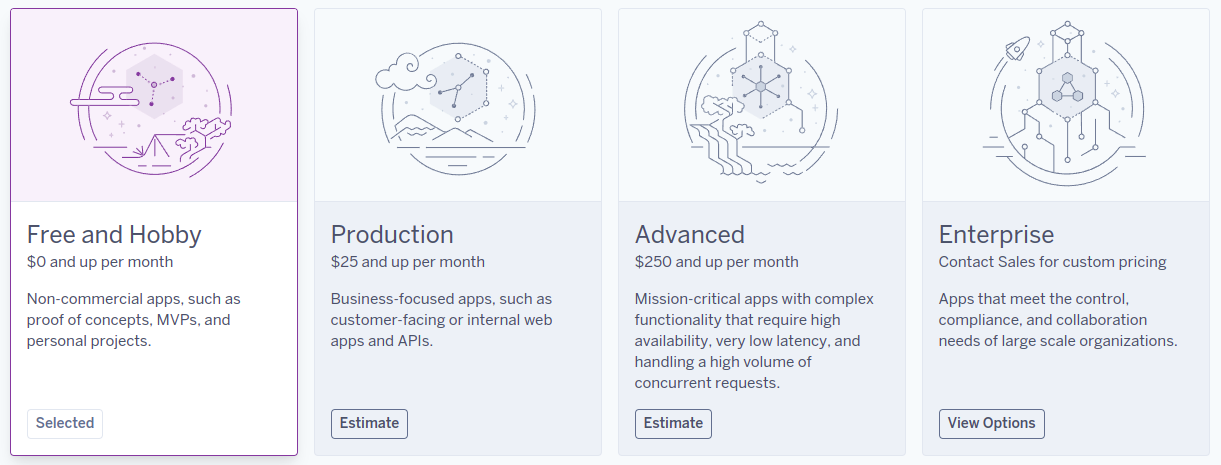
\includegraphics[width=1.0\textwidth]{imagenes/05_Gestion/planes_heroku.png}
\begin{center}
Fuente: \url{https://www.heroku.com/pricing}
\end{center}
\caption{Planes de pago sobre las apps de Heroku}
\label{fig:planes_app_heroku}
\end{figure}

\begin{figure}[H]
\centering
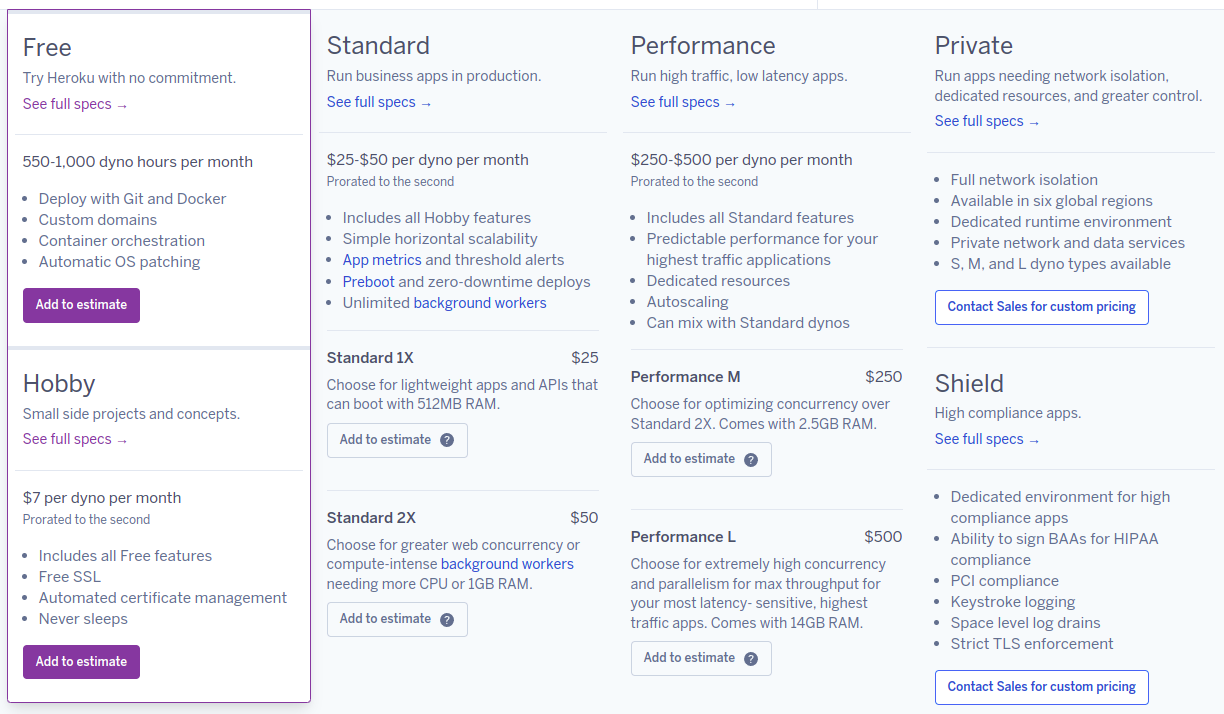
\includegraphics[width=1.0\textwidth]{imagenes/05_Gestion/planes_dynos_heroku.png}
\begin{center}
Fuente: \url{https://www.heroku.com/pricing}
\end{center}
\caption{Planes de pago sobre los dynos de Heroku}
\label{fig:planes_dynos_heroku}
\end{figure}

\begin{figure}[H]
\centering
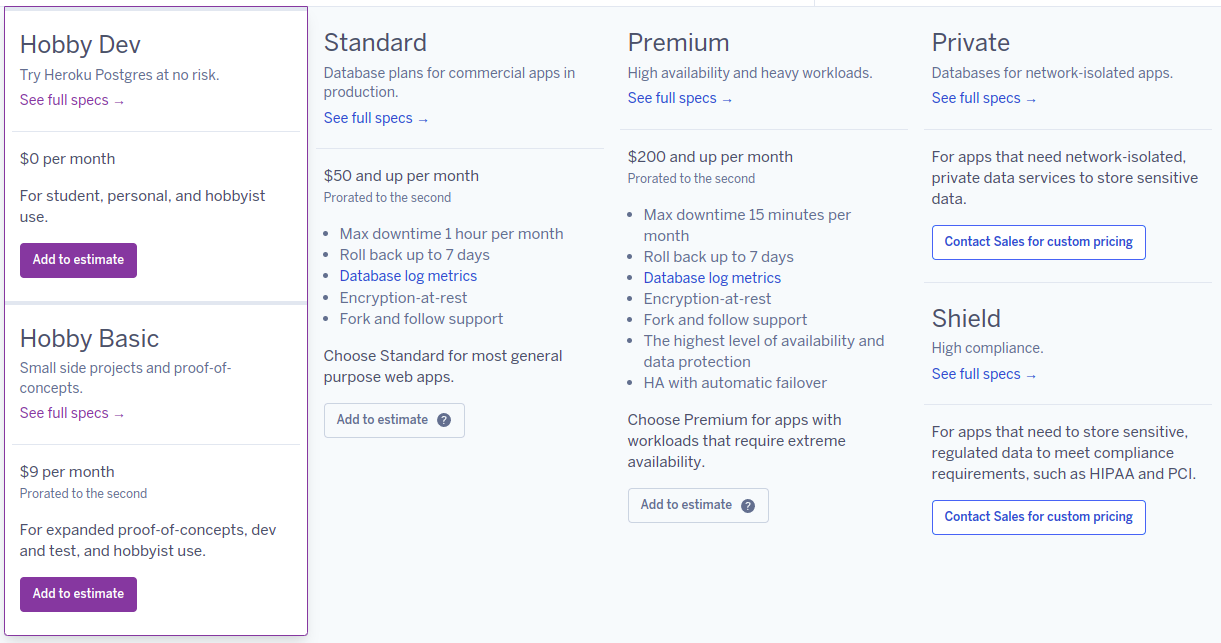
\includegraphics[width=1.0\textwidth]{imagenes/05_Gestion/planes_postgres_heroku.png}
\begin{center}
Fuente: \url{https://www.heroku.com/pricing}
\end{center}
\caption{Planes de pago sobre las bases de datos de Heroku}
\label{fig:planes_postgres_heroku}
\end{figure}

\item \textbf{BlenderBot}: Es una herramienta de software libre para la creación del chatbot.
\item \textbf{Dialogflow}: Es una herramienta para el despliegue del chatbot. Se hará uso de la versión gratuita de la herramienta.
\item \textbf{SweetAlert2}: SweetAlert es un plugin de jQuery y con el cual podremos dar un aspecto profesional a los mensajes que lancemos a los usuarios acorde a las tendencias actuales. Además, tenemos la posibilidad de configurar el plugin de muchas formas diferentes.
\item \textbf{Docker}: Docker es un proyecto de código abierto que automatiza el despliegue de aplicaciones dentro de contenedores de software, proporcionando una capa adicional de abstracción y automatización de virtualización de aplicaciones en múltiples sistemas operativos.
\item \textbf{Uvicorn}: Uvicorn es una implementación de servidor web ASGI para Python.
\item \textbf{FastAPI}: FastAPI es un marco de trabajo moderno, rápido (de alto rendimiento), para la construcción de API's con Python 3.6+ basado en sugerencias de tipo estándar de Python.
\item \textbf{Ngrok}: Ngrok es un servicio que nos permite crear nuestro servidor local en un subdominio para poder visualizarlo fuera de la LAN, a través de internet.
\end{itemize}

\subsection{Recursos de comunicación y documentación} \label{subsec:recur_comu_docu}

Todo buen proyecto debe ser resultado de una buena comunicación entre su personal. Además, se debe elaborar una documentación de calidad para conseguir que el proyecto sea accesible por personas ajenas al desarrollo del proyecto. Para conseguir estos objetivos se ha hecho uso de varias herramientas, entre las cuales se encuentran las siguientes:

\begin{itemize}
\item \textbf{Google Meet}: Es un servicio de videotelefonía desarrollado por Google. Este servicio se ha utilizado para realizar las distintas reuniones con el tutor.
\item \textbf{Correo UGR}: Es un servicio de correo electrónico de la UGR. Este servicio se ha utilizado para realizar conversaciones con el tutor sobre temas puntuales o de menor peso.
\item \textbf{Overleaf}: Es una plataforma de edición de documentos escritos en LaTeX. Esta plataforma se ha usado para la elaboración de la documentación del proyecto.
\item \textbf{Texmaker}: Es un editor empleado para desarrollar documentos con LaTeX.
\item \textbf{Visual Paradigm}: Es una herramienta de modelado de diagramas de desarrollo software. En principio es una herramienta de pago, pero la UGR dispone de licencias de uso educativo para los estudiantes.
\item \textbf{Microsoft Powerpoint}: Es un programa de presentación desarrollado por Microsoft. Con este programa se ha elaborado la presentación del proyecto.
\end{itemize}



\section{Gestión de costes}

Todo proyecto debe tener su gestión de costes para evaluar la viabilidad económica del proyecto. En la gestión de costes se tiene en cuenta el coste derivado de cada uno de los recursos citados en el apartado \ref{sec:gest_recursos}.

\subsection{Costes de recursos humanos}

Los costes de recursos humanos vienen derivados del trabajo realizado por el equipo de desarrollo, como en este proyecto este equipo está formado por una única persona, el alumno, el coste de recursos humanos será el equivalente al trabajo realizado por un ingeniero informático durante el desarrollo del proyecto, es decir, se simula que el alumno se trata de un ingeniero informático que trabaja de forma autónoma.

Para estimar este coste de recursos humanos es necesario estimar el coste de ese trabajo y para ello es necesario recabar información.

En primer lugar, es necesario calcular el tiempo que ha estado trabajando el ingeniero. Dado que el proyecto tiene una duración de 5 meses.

\begin{center}
$Dias\ totales\ =\ 5\ meses\ *\ 30\ dias / mes\ =\ 150\ dias$
\end{center}

El tiempo total aproximado será de 150 días. A este tiempo total habrá que descontar los días no laborables. Los días no laborables en estos 5 meses serían aproximadamente:

\begin{center}
$Dias\ no\ laborables\ =\ 5\ meses\ *\ 8\ dias/mes\ =\ 40\ dias$
\end{center}

Por lo tanto, los días laborables gastados por el trabajador son:

\begin{center}
$Dias\ laborables\ =\ Dias\ totales\ -\ Dias\ no\ laborables\ =\ 110\ dias$
\end{center}

Además, dentro de cada día laborable hay una jornada laboral. Normalmente, esta jornada es de 8 horas, pero como el desarrollo del proyecto se ha hecho en conjunto con la realización de otras asignaturas, no se ha dispuesto de todo el tiempo, por lo tanto, se estimará que aproximadamente se ha trabajado unas 5 horas al día. En consecuencia, el número total de horas trabajadas es el siguiente:

\begin{center}
$Horas\ laborables\ =\ Dias\ laborables\ *\ 5\ horas/dia\ =\ 550\ horas$
\end{center}

Este número de horas excede en gran medida el número de horas correspondientes a los \gls{ECTS} de un TFG. El número mínimo de horas que se debe emplear en el desarrollo de un TFG deben ser 300 horas.

Una vez tenemos el tiempo trabajado por el ingeniero, es necesario obtener que salario tiene este trabajador a la hora. Para obtener esta información me he basado en el estudio de la página talent.com \footnote{\url{https://acortar.link/MiqarT}}. En este estudio se analiza el sueldo medio de un ingeniero informático en España, el salario medio es de 2.208 \EURtm al mes. Por lo tanto, el salario medio por hora será de 13,59 \EURtm.

Con la información recabada ya podemos estimar el coste del trabajo realizado por el ingeniero. El coste total se puede ver en la Tabla \ref{tab:coste_recur_humanos}.

\begin{table}[h]
\centering
\resizebox{\textwidth}{!}{%
\begin{tabular}{@{}cccc@{}}
\toprule
\textbf{Recurso} & \textbf{Precio / Hora}             & \textbf{Nº Horas}    & \textbf{Importe}              \\ \midrule
Trabajo autónomo  & 13,59 \EURtm / hora & 550                  & 7474,50 \EURtm \\ \midrule
\textbf{Total:}   & \multicolumn{1}{l}{}               & \multicolumn{1}{l}{} & 7474,50 \EURtm \\ \bottomrule
\end{tabular}%
}
\caption{Costes asociados a los recursos humanos}
\label{tab:coste_recur_humanos}
\end{table}

\subsection{Costes de recursos materiales}

Los costes derivados de los recursos materiales se calculan de una forma distinta a la realizada en los costes de recursos humanos, por la simple razón de que los recursos materiales se van devaluando con el paso del tiempo tras su adquisición. Por esta razón deberemos calcular el coste de los distintos recursos materiales con la depreciación aplicada.

Para calcular el coste actual del recurso se debe obtener previamente la siguiente información:

\begin{itemize}
\item Coste de adquisición del producto
\item Coste residual del producto, es decir, el valor del producto al final de su vida útil
\item Coeficiente de amortiguación lineal
\end{itemize}

Nos vamos a centrar en el portátil personal, ya que a pesar de que los servidores GPU del Instituto DaSCI tienen un coste de uso, al ser estudiantes de la UGR el coste para nuestro proyecto ha sido nulo y de esta forma lo hemos indicado en el cálculo de los costes; y en el caso de usar servidores en la nube ajenos a la UGR, el coste de estos servidores suele tener un coste fijo cada mes a través de una cuota mensual o en ocasiones el coste de estos servidores se calcula según el tiempo de uso que se haya hecho de estos servidores.

El coste de adquisición del producto es de 1100 \EURtm. Como coste residual fijamos la cantidad de 100 \EURtm. Y por último queda fijar el coeficiente de amortiguación lineal, para fijar este valor he recabado información sobre el coeficiente de amortiguación lineal de los equipos electrónicos. Esta información la encontré en un artículo de la página web Iberley \footnote{\url{https://www.iberley.es/temas/tablas-amortizacion-i-sociedades-30681}}, donde se indica que el coeficiente de amortiguación lineal máximo para estos equipos electrónicos es del 20\%.

Para calcular el coste actual del producto se utiliza la siguiente fórmula:

\begin{center}
$C_{ac}\ =\ (C_{ad}\ -\ C_{re})\ *\ C_{amor}$\\
$C_{ac}:\ Coste\ actual$\\
$C_{ad}:\ Coste\ adquisicion$\\
$C_{re}:\ Coste\ residual$\\
$C_{amor}:\ Coeficiente\ amortiguacion$
\end{center}

Siguiendo esta fórmula, el coste actual del portátil es de 200 \EURtm. Pero este coste indica el coste anual del recurso, por lo que habrá que calcular el coste del recurso teniendo en cuenta el tiempo de empleo. El tiempo de uso es el mismo que el tiempo trabajado por el alumno, es decir, 5 meses trabajando los 5 días laborables de la semana a razón de 5 horas por día. Basándonos en los cálculos del anterior apartado, el total de horas laborables es de 550 horas. Por lo que el coste final del portátil es el siguiente:

\begin{center}
$Coste\ final\ =\ 200\ *\ \frac{550}{1200}\ =\ 91,66\ euros$
\end{center}

Al igual que se hace con los costes asociados a los recursos humanos, en este caso se puede ver un resumen de los costes asociados a los recursos materiales en la Tabla \ref{tab:coste_recur_materiales}.

\begin{table}[h]
\centering
\resizebox{\textwidth}{!}{%
\begin{tabular}{@{}cccc@{}}
\toprule
\textbf{Recurso}  & \textbf{Precio / Hora}            & \textbf{Nº Horas}    & \textbf{Importe}            \\ \midrule
Portátil personal & 0,16 \EURtm / hora & 550                  & 91,66 \EURtm \\ \midrule
\textbf{Total:}   & \multicolumn{1}{l}{}              & \multicolumn{1}{l}{} & 91,66 \EURtm \\ \bottomrule
\end{tabular}%
}
\caption{Costes asociados a los recursos materiales}
\label{tab:coste_recur_materiales}
\end{table}

\subsection{Costes de recursos software}

En este apartado se estima el coste de todos los recursos software listados en el apartado \ref{subsec:recur_software}. Tal y como se indica en este apartado, todos los recursos software utilizados son de software libre, y en concreto con Heroku, aunque no es un software gratuito, sí que dispone de una versión gratuita que tiene ciertas limitaciones, pero que nos sirve para el desarrollo del proyecto.

\subsection{Costes de recursos de comunicación y documentación}

En este apartado se estima el coste de todos los recursos para la comunicación con la tutora y la elaboración de la documentación. Al igual que pasa con el apartado anterior, tal y como se indica en el apartado \ref{subsec:recur_comu_docu}, todos los recursos empleados son de software libre, aunque hace falta puntualizar que la herramienta Visual Paradigm es de pago, pero como la UGR dispone de licencias gratuitas para los alumnos, se ha aprovechado esta ventaja para la elaboración de los diagramas del diseño del proyecto.

\subsection{Costes adicionales}

Dentro de los costes adicionales se tiene el coste derivado de todos aquellos recursos que no hayan sido listados en ninguno de los anteriores apartados. Los principales recursos de este apartado son el Internet y la factura de la luz. La tarifa de Internet contratada tiene un coste de 30 \EURtm/mes, por lo tanto, el coste total por el Internet asciende a 150 \EURtm. Y en cuanto a la factura de la luz, es un coste más difícil de calcular, dado que hay muchas variables que intervienen en su valor, pero una posible estimación sobre su valor podría ser 25 \EURtm. El coste total derivado de estos recursos adicionales se puede ver en la Tabla \ref{tab:coste_recur_adicionales}.

\begin{table}[h]
\centering
\resizebox{0.5\textwidth}{!}{%
\begin{tabular}{@{}cc@{}}
\toprule
\textbf{Recurso}  & \textbf{Importe}             \\ \midrule
Internet          & 150,00 \EURtm \\ \midrule
Factura de la luz & 25,00 \EURtm  \\ \midrule
\textbf{Total:}   & 175,00 \EURtm \\ \bottomrule
\end{tabular}%
}
\caption{Costes asociados a los recursos adicionales}
\label{tab:coste_recur_adicionales}
\end{table}



\section{Presupuesto total}

Para tener una visión global de todos los costes analizados se ha elaborado una tabla donde se desglosa toda la información de cada apartado y finalmente se calcula el coste acumulado de todo el proyecto. Estos datos se pueden ver en la Tabla \ref{tab:presupuesto_total}.


\begin{longtable}[c]{lr}
\hline
\textbf{Recurso}                     & \textbf{Importe}                       \\
\endfirsthead
%
\endhead
%
\hline
\endfoot
%
\endlastfoot
%
                                     &                                        \\ \hline
\textbf{Costes de recursos humanos}  & \textbf{7474,50 \EURtm} \\
                                     & \multicolumn{1}{l}{}                   \\
Trabajo autónomo                     & 7474,50 \EURtm          \\ \hline
\textbf{Costes de recursos materiales}                      & \textbf{91,66 \EURtm} \\
                                     & \multicolumn{1}{l}{}                   \\
Portátil personal                    & 91,66 \EURtm            \\
Servidores GPU de la UGR             & 0,00 \EURtm             \\ \hline
\textbf{Costes de recursos software} & \textbf{0,00 \EURtm}    \\
                                     & \multicolumn{1}{l}{}                   \\
Sistema Operativo                    & 0,00 \EURtm             \\
GitHub                               & 0,00 \EURtm             \\
Git                                  & 0,00 \EURtm             \\
Visual Studio Code                   & 0,00 \EURtm             \\
Heroku                               & 0,00 \EURtm             \\
BlenderBot                           & 0,00 \EURtm             \\
Dialogflow                           & 0,00 \EURtm             \\
SweetAlert2                          & 0,00 \EURtm             \\
Docker                               & 0,00 \EURtm             \\
Uvicorn                              & 0,00 \EURtm             \\
FastAPI                              & 0,00 \EURtm             \\
Ngrok                                & 0,00 \EURtm             \\ \hline
\textbf{Costes de recursos de comunicación y documentación} & \textbf{0,00 \EURtm}  \\
                                     & \multicolumn{1}{l}{}                   \\
Google Meet                          & 0,00 \EURtm             \\
Correo UGR                           & 0,00 \EURtm             \\
Overleaf                             & 0,00 \EURtm             \\
Texmaker                             & 0,00 \EURtm             \\
Visual Paradigm                      & 0,00 \EURtm             \\
Microsoft Powerpoint                 & 0,00 \EURtm             \\ \hline
\textbf{Costes adicionales}          & \textbf{175,00 \EURtm}  \\
                                     & \multicolumn{1}{l}{}                   \\
Internet                             & 150,00 \EURtm           \\
Factura de la luz                    & 25,00 \EURtm            \\
                                     & \multicolumn{1}{l}{}                   \\ \hline
\multicolumn{1}{r}{\textbf{Total:}}  & \textbf{7741,16 \EURtm} \\ \hline
\caption{Presupuesto total del proyecto}
\label{tab:presupuesto_total}
\end{longtable}


























\chapter{Diseño}








\chapter{Implementación}





\chapter{Pruebas}





\chapter{Conclusiones y posibles ampliaciones}

El objetivo del proyecto era implementar un chatbot, con la capacidad de realizar acciones didácticas sobre un abanico de temas a través del establecimiento de una conversación con un usuario del sistema, y que pudiera ser usado en eventos como La Noche Europea de l@s Investigador@s.

Los conocimientos empleados para el desarrollo del proyecto están basados en los conocimientos adquiridos en un gran abanico de asignaturas del \href{https://grados.ugr.es/informatica/pages/infoacademica/estudios}{Plan de Estudios} del Grado en Ingeniería Informática como son \textit{Fundamentos de Bases de Datos, Fundamentos de Ingeniería del Software, Aprendizaje Automático, Procesadores de Lenguajes, Visión por computador, Programación Técnica y Científica y Estructuras de Datos}.

Basándonos en los resultados obtenidos en las pruebas del Apartado \ref{pruebas}, podríamos decir que se han efectuado todas las tareas de las historias de usuario planteadas en el Apartado \ref{sec:historias_usuario} para considerar que se han cumplido sus objetivos en su mayoría. Con la salvedad de la HU.7 (Tabla \ref{tab:HU7}), la cual hace referencia al comportamiento del chatbot a la hora de orientar la respuesta del mismo hacia la temática del chatbot de una forma didáctica. Basándonos en los resultados de las pruebas en la generación de respuestas, vemos como le cuesta al modelo realizar esta tarea didáctica, por lo tanto, no se puede afirmar el cumplimiento de esta historia de usuario. Aunque esto no quiere decir que el chatbot sea capaz de entablar una conversación con el usuario, la cual trascurre con cierta coherencia y no de forma aleatoria.

Pero quitando esta última historia de usuario, el resto de historias de usuario considero que se han cumplido con creces. Por ejemplo, la deducción de la edad del usuario se ha resuelto de manera sencilla y rápida mediante un modelo pre entrenado, que como se ha visto en las pruebas, da unos buenos resultados en la mayoría de situaciones. Por su puesto no siempre acierta, ya que en ocasiones el aspecto de una persona no está asociado con su edad real, esto forma parte de la complejidad de extraer información del aspecto humano. Aunque teniendo estos fallos, pienso que es una solución práctica, que evita la complejidad que podría suponer un análisis del lenguaje del usuario, para lo cual sería necesario un tiempo y unos conocimientos difícilmente alcanzables en el desarrollo de este proyecto. Y otro de los grandes logros es la obtención de una interfaz totalmente funcional y con ciertos elementos que la hagan un poco más atractiva como el modo oscuro y la interfaz responsive.

A pesar de que la HU.7 es una de las más importantes a la hora de desarrollar el proyecto, tal y como se indica en la Tabla \ref{tab:listado_HU}; no se puede considerar que el proyecto haya sido todo un fracaso, ya que el desarrollo de un chatbot tan complejo es una tarea muy difícil. Por supuesto, este fracaso en el cumplimiento de la HU.7 viene derivado de la materialización del riesgo de fijar objetivos pocos realistas. Está claro que no es un objetivo imposible, pero si difícilmente alcanzable en el periodo de tiempo disponible para el desarrollo de este proyecto.

Algo que hay que recalcar es que aunque no se haya conseguido un chatbot didáctico, no quiere decir que no se haya trabajado en el proyecto. Como ya se indicó en el apartado de gestión, se han invertido un número mayor de horas de las que requiere como mínimo un TFG. Durante estas horas se han adquirido una cantidad ingente de conocimientos, ya que casi todas las tecnologías usadas en el proyecto eran desconocidas, exceptuando la plataforma Github, ciertos conocimientos sobre los contenedores, y la herramienta Overleaf, así como una base en el lenguaje \textit{LaTeX}. Pero, por otro lado, he realizado tareas cuyos conocimientos requeridos no habían sido vistos en todo el grado.

Una de las primeras tareas que me hizo ponerme a investigar sobre el ámbito de las páginas web, fue la elaboración de una interfaz web para nuestro sistema. Durante esta investigación se adquirieron muchos conocimientos en el lenguaje HTML, Javascript y CSS. Y la adquisición de conocimientos no se quedó en lo teórico, sino que se puso en práctica enlazando elementos implementados en los distintos lenguajes y obteniendo un producto final con grandes posibilidades.

Otro punto que me empujó a investigar mucho fue la implementación del servidor del Controlador, ya que tuve que utilizar el framework FastAPI, el cual era totalmente desconocido para mí. Estos conocimientos también me ayudaron con el servidor del Modelo porque se basan en el mismo framework.

Y por último, una de las partes que aunque en principio parezca que no llevan mucho trabajo, internamente si lo llevan. Esta parte son los modelos empleados para realizar la deducción de edad o la generación de respuestas. Aunque se hayan usado modelos pre entrenados, se han utilizado modelos basados en Transformers, los cuales no había utilizado nunca porque solamente había usado modelos basados en convoluciones para la asignatura de \textit{Visión por computador}. Además, son modelos implementados con PyTorch y hasta el momento únicamente había trabajado con TensorFlow. Y también que sean modelo pre entrenados no implica que no haya que trabajar con ellos y, por tanto, se debe aprender como funcionan estos modelos y por supuesto, como funciona la plataforma Huggingface que es la que contiene los modelos pre entrenados.

En definitiva, este proyecto ha sido todo un reto para mí, ya que se han puesto a prueba todos mis conocimientos adquiridos durante el grado y capacidades para adaptarme, puesto que he desarrollado un sistema desde la parte más visible como es el frontend y la parte más oculta y lógica del sistema como es el backend.

Por último, la reflexión final es que el sistema implementado es un sistema que cumple con muchos de sus objetivos, pero que sigue teniendo mucho potencial por explotar si se invierte un poco más de tiempo en él.

\section{Posibles ampliaciones}

Como se ha ido indicando en esta parte final de la memoria, el proyecto tiene claras vías por donde ampliar y mejorar el proyecto. Algunas de las posibles ampliaciones son las siguientes:

\begin{itemize}
\item \textbf{Búsqueda y utilización de una plataforma de despliegue con GPU:} Si utilizamos una plataforma que tenga las características y las funcionalidades que tiene Heroku, junto con la posibilidad de utilizar una GPU, podríamos realizar una reestructuración del sistema la cual simplificaría esta estructura. La simplificación conllevaría la unión de los servidores del Controlador y del Modelo, y una refactorización completa del código. Esta unión evita el trabajo extra derivado de implementar dos servidores y de tener que mantenerlos en funcionamiento y actualizados por separado, teniendo partes en común. Además, la unión elimina muchos envíos de peticiones entre servidores, ya que el intercambio de información entre el Controlador y el Modelo se efectuarían de forma interna, lo que conlleva mayor rapidez y seguridad.
\item \textbf{Mejora de la interfaz web:} Basándonos en el feedback de los usuarios que ejecutaron las pruebas de la interfaz web, se podría modernizar la interfaz web empleando herramientas más actuales para implementar la funcionalidad de la interfaz, y que esta tome un aspecto más renovado.
\item \textbf{Seguir con la obtención de información:} Como se ha indicado en varios de los apartados de la memoria, es necesario avanzar en la obtención de información para intentar que el chatbot adquiera un tono didáctico.
\item \textbf{Reutilización de los resultados:} Un chatbot nunca deja de mejorarse, ya que normalmente se reutilizan los resultados de conversaciones realizadas con el chatbot para mejorar al mismo. Nuestro sistema ya es capaz de guardar las conversaciones realizadas con el chatbot en una base de datos, pero nos falta un programa que sea capaz de mover esa información y entrenar al chatbot con ella. Además, sería muy interesante que se puede automatizar este proceso, ya que evitaría mucha carga de trabajo para el administrador del sistema.
\item \textbf{Mejorar el modelo de deducción de edad:} Aunque como se ha visto en las pruebas del modelo de deducción tiene una calidad más que aceptable para nuestro sistema, siempre se puede mejorar porque se trata de un modelo pre entrenado. Por lo tanto, podríamos entrenar al modelo con muchas más imágenes que podemos obtener de las múltiples bases de imágenes existentes en internet. Claramente, esto conlleva una carga de trabajo tremenda, ya que se deben obtener las imágenes, etiquetarlas si no lo están, y por último crear un programa para el entrenamiento del modelo pre entrenado.
\item \textbf{Creación de una interfaz propia para el chatbot:} La creación de una interfaz propia podría ayudar a seguir avanzando en la simplificación del sistema, por el hecho de que ahora mismo se deben generar secciones distintas para cada rango de edad que distingue el sistema. Estas duplicidades vienen derivadas del uso de la interfaz de Dialogflow. Por lo tanto, una gran mejora sería crear nuestra propia interfaz web para eliminar todas estas duplicidades y poder simplificar el sistema. Además, tendríamos un mayor control del sistema. Incluso se podría dejar de hacer uso de Dialogflow, aunque esto conllevaría un mayor trabajo dado que eliminamos las facilidades que nos da Dialogflow a la hora de desplegar el chatbot.
\item \textbf{Uso de un avatar:} Actualmente se está poniendo de moda producir chatbots con una interfaz visual compuesta por un avatar. Este avatar tiene un aspecto humano para hacer más cómodo el establecimiento de las conversaciones. Con este avatar eliminamos la idea antigua de tener una interfaz textual para poder interactuar con el chatbot.
\end{itemize}




\nocite{*}
\bibliographystyle{IEEEtran}
\bibliography{
    bibliografia/planificacion, 
    bibliografia/analisis,
    bibliografia/glosario
}
\addcontentsline{toc}{chapter}{Bibliografía}


%
%%\chapter{Conclusiones y Trabajos Futuros}
%
%


%
\appendix
%\chapter{Manual de usuario}
%%\input{apendices/paper/paper}

\addcontentsline{toc}{chapter}{Glosario}
\printglossary
\chapter*{}
\thispagestyle{empty}

\end{document}
